\documentclass[11pt]{article}

    \usepackage[breakable]{tcolorbox}
    \usepackage{parskip} % Stop auto-indenting (to mimic markdown behaviour)
    
    \usepackage{iftex}
    \ifPDFTeX
    	\usepackage[T1]{fontenc}
    	\usepackage{mathpazo}
    \else
    	\usepackage{fontspec}
    \fi

    % Basic figure setup, for now with no caption control since it's done
    % automatically by Pandoc (which extracts ![](path) syntax from Markdown).
    \usepackage{graphicx}
    % Maintain compatibility with old templates. Remove in nbconvert 6.0
    \let\Oldincludegraphics\includegraphics
    % Ensure that by default, figures have no caption (until we provide a
    % proper Figure object with a Caption API and a way to capture that
    % in the conversion process - todo).
    \usepackage{caption}
    \DeclareCaptionFormat{nocaption}{}
    \captionsetup{format=nocaption,aboveskip=0pt,belowskip=0pt}

    \usepackage[Export]{adjustbox} % Used to constrain images to a maximum size
    \adjustboxset{max size={0.9\linewidth}{0.9\paperheight}}
    \usepackage{float}
    \floatplacement{figure}{H} % forces figures to be placed at the correct location
    \usepackage{xcolor} % Allow colors to be defined
    \usepackage{enumerate} % Needed for markdown enumerations to work
    \usepackage{geometry} % Used to adjust the document margins
    \usepackage{amsmath} % Equations
    \usepackage{amssymb} % Equations
    \usepackage{textcomp} % defines textquotesingle
    % Hack from http://tex.stackexchange.com/a/47451/13684:
    \AtBeginDocument{%
        \def\PYZsq{\textquotesingle}% Upright quotes in Pygmentized code
    }
    \usepackage{upquote} % Upright quotes for verbatim code
    \usepackage{eurosym} % defines \euro
    \usepackage[mathletters]{ucs} % Extended unicode (utf-8) support
    \usepackage{fancyvrb} % verbatim replacement that allows latex
    \usepackage{grffile} % extends the file name processing of package graphics 
                         % to support a larger range
    \makeatletter % fix for grffile with XeLaTeX
    \def\Gread@@xetex#1{%
      \IfFileExists{"\Gin@base".bb}%
      {\Gread@eps{\Gin@base.bb}}%
      {\Gread@@xetex@aux#1}%
    }
    \makeatother

    % The hyperref package gives us a pdf with properly built
    % internal navigation ('pdf bookmarks' for the table of contents,
    % internal cross-reference links, web links for URLs, etc.)
    \usepackage{hyperref}
    % The default LaTeX title has an obnoxious amount of whitespace. By default,
    % titling removes some of it. It also provides customization options.
    \usepackage{titling}
    \usepackage{longtable} % longtable support required by pandoc >1.10
    \usepackage{booktabs}  % table support for pandoc > 1.12.2
    \usepackage[inline]{enumitem} % IRkernel/repr support (it uses the enumerate* environment)
    \usepackage[normalem]{ulem} % ulem is needed to support strikethroughs (\sout)
                                % normalem makes italics be italics, not underlines
    \usepackage{mathrsfs}
    

    
    % Colors for the hyperref package
    \definecolor{urlcolor}{rgb}{0,.145,.698}
    \definecolor{linkcolor}{rgb}{.71,0.21,0.01}
    \definecolor{citecolor}{rgb}{.12,.54,.11}

    % ANSI colors
    \definecolor{ansi-black}{HTML}{3E424D}
    \definecolor{ansi-black-intense}{HTML}{282C36}
    \definecolor{ansi-red}{HTML}{E75C58}
    \definecolor{ansi-red-intense}{HTML}{B22B31}
    \definecolor{ansi-green}{HTML}{00A250}
    \definecolor{ansi-green-intense}{HTML}{007427}
    \definecolor{ansi-yellow}{HTML}{DDB62B}
    \definecolor{ansi-yellow-intense}{HTML}{B27D12}
    \definecolor{ansi-blue}{HTML}{208FFB}
    \definecolor{ansi-blue-intense}{HTML}{0065CA}
    \definecolor{ansi-magenta}{HTML}{D160C4}
    \definecolor{ansi-magenta-intense}{HTML}{A03196}
    \definecolor{ansi-cyan}{HTML}{60C6C8}
    \definecolor{ansi-cyan-intense}{HTML}{258F8F}
    \definecolor{ansi-white}{HTML}{C5C1B4}
    \definecolor{ansi-white-intense}{HTML}{A1A6B2}
    \definecolor{ansi-default-inverse-fg}{HTML}{FFFFFF}
    \definecolor{ansi-default-inverse-bg}{HTML}{000000}

    % commands and environments needed by pandoc snippets
    % extracted from the output of `pandoc -s`
    \providecommand{\tightlist}{%
      \setlength{\itemsep}{0pt}\setlength{\parskip}{0pt}}
    \DefineVerbatimEnvironment{Highlighting}{Verbatim}{commandchars=\\\{\}}
    % Add ',fontsize=\small' for more characters per line
    \newenvironment{Shaded}{}{}
    \newcommand{\KeywordTok}[1]{\textcolor[rgb]{0.00,0.44,0.13}{\textbf{{#1}}}}
    \newcommand{\DataTypeTok}[1]{\textcolor[rgb]{0.56,0.13,0.00}{{#1}}}
    \newcommand{\DecValTok}[1]{\textcolor[rgb]{0.25,0.63,0.44}{{#1}}}
    \newcommand{\BaseNTok}[1]{\textcolor[rgb]{0.25,0.63,0.44}{{#1}}}
    \newcommand{\FloatTok}[1]{\textcolor[rgb]{0.25,0.63,0.44}{{#1}}}
    \newcommand{\CharTok}[1]{\textcolor[rgb]{0.25,0.44,0.63}{{#1}}}
    \newcommand{\StringTok}[1]{\textcolor[rgb]{0.25,0.44,0.63}{{#1}}}
    \newcommand{\CommentTok}[1]{\textcolor[rgb]{0.38,0.63,0.69}{\textit{{#1}}}}
    \newcommand{\OtherTok}[1]{\textcolor[rgb]{0.00,0.44,0.13}{{#1}}}
    \newcommand{\AlertTok}[1]{\textcolor[rgb]{1.00,0.00,0.00}{\textbf{{#1}}}}
    \newcommand{\FunctionTok}[1]{\textcolor[rgb]{0.02,0.16,0.49}{{#1}}}
    \newcommand{\RegionMarkerTok}[1]{{#1}}
    \newcommand{\ErrorTok}[1]{\textcolor[rgb]{1.00,0.00,0.00}{\textbf{{#1}}}}
    \newcommand{\NormalTok}[1]{{#1}}
    
    % Additional commands for more recent versions of Pandoc
    \newcommand{\ConstantTok}[1]{\textcolor[rgb]{0.53,0.00,0.00}{{#1}}}
    \newcommand{\SpecialCharTok}[1]{\textcolor[rgb]{0.25,0.44,0.63}{{#1}}}
    \newcommand{\VerbatimStringTok}[1]{\textcolor[rgb]{0.25,0.44,0.63}{{#1}}}
    \newcommand{\SpecialStringTok}[1]{\textcolor[rgb]{0.73,0.40,0.53}{{#1}}}
    \newcommand{\ImportTok}[1]{{#1}}
    \newcommand{\DocumentationTok}[1]{\textcolor[rgb]{0.73,0.13,0.13}{\textit{{#1}}}}
    \newcommand{\AnnotationTok}[1]{\textcolor[rgb]{0.38,0.63,0.69}{\textbf{\textit{{#1}}}}}
    \newcommand{\CommentVarTok}[1]{\textcolor[rgb]{0.38,0.63,0.69}{\textbf{\textit{{#1}}}}}
    \newcommand{\VariableTok}[1]{\textcolor[rgb]{0.10,0.09,0.49}{{#1}}}
    \newcommand{\ControlFlowTok}[1]{\textcolor[rgb]{0.00,0.44,0.13}{\textbf{{#1}}}}
    \newcommand{\OperatorTok}[1]{\textcolor[rgb]{0.40,0.40,0.40}{{#1}}}
    \newcommand{\BuiltInTok}[1]{{#1}}
    \newcommand{\ExtensionTok}[1]{{#1}}
    \newcommand{\PreprocessorTok}[1]{\textcolor[rgb]{0.74,0.48,0.00}{{#1}}}
    \newcommand{\AttributeTok}[1]{\textcolor[rgb]{0.49,0.56,0.16}{{#1}}}
    \newcommand{\InformationTok}[1]{\textcolor[rgb]{0.38,0.63,0.69}{\textbf{\textit{{#1}}}}}
    \newcommand{\WarningTok}[1]{\textcolor[rgb]{0.38,0.63,0.69}{\textbf{\textit{{#1}}}}}
    
    
    % Define a nice break command that doesn't care if a line doesn't already
    % exist.
    \def\br{\hspace*{\fill} \\* }
    % Math Jax compatibility definitions
    \def\gt{>}
    \def\lt{<}
    \let\Oldtex\TeX
    \let\Oldlatex\LaTeX
    \renewcommand{\TeX}{\textrm{\Oldtex}}
    \renewcommand{\LaTeX}{\textrm{\Oldlatex}}
    % Document parameters
    % Document title
    \title{QF205-Compiled-Report}
    
    
    
    
    
% Pygments definitions
\makeatletter
\def\PY@reset{\let\PY@it=\relax \let\PY@bf=\relax%
    \let\PY@ul=\relax \let\PY@tc=\relax%
    \let\PY@bc=\relax \let\PY@ff=\relax}
\def\PY@tok#1{\csname PY@tok@#1\endcsname}
\def\PY@toks#1+{\ifx\relax#1\empty\else%
    \PY@tok{#1}\expandafter\PY@toks\fi}
\def\PY@do#1{\PY@bc{\PY@tc{\PY@ul{%
    \PY@it{\PY@bf{\PY@ff{#1}}}}}}}
\def\PY#1#2{\PY@reset\PY@toks#1+\relax+\PY@do{#2}}

\expandafter\def\csname PY@tok@w\endcsname{\def\PY@tc##1{\textcolor[rgb]{0.73,0.73,0.73}{##1}}}
\expandafter\def\csname PY@tok@c\endcsname{\let\PY@it=\textit\def\PY@tc##1{\textcolor[rgb]{0.25,0.50,0.50}{##1}}}
\expandafter\def\csname PY@tok@cp\endcsname{\def\PY@tc##1{\textcolor[rgb]{0.74,0.48,0.00}{##1}}}
\expandafter\def\csname PY@tok@k\endcsname{\let\PY@bf=\textbf\def\PY@tc##1{\textcolor[rgb]{0.00,0.50,0.00}{##1}}}
\expandafter\def\csname PY@tok@kp\endcsname{\def\PY@tc##1{\textcolor[rgb]{0.00,0.50,0.00}{##1}}}
\expandafter\def\csname PY@tok@kt\endcsname{\def\PY@tc##1{\textcolor[rgb]{0.69,0.00,0.25}{##1}}}
\expandafter\def\csname PY@tok@o\endcsname{\def\PY@tc##1{\textcolor[rgb]{0.40,0.40,0.40}{##1}}}
\expandafter\def\csname PY@tok@ow\endcsname{\let\PY@bf=\textbf\def\PY@tc##1{\textcolor[rgb]{0.67,0.13,1.00}{##1}}}
\expandafter\def\csname PY@tok@nb\endcsname{\def\PY@tc##1{\textcolor[rgb]{0.00,0.50,0.00}{##1}}}
\expandafter\def\csname PY@tok@nf\endcsname{\def\PY@tc##1{\textcolor[rgb]{0.00,0.00,1.00}{##1}}}
\expandafter\def\csname PY@tok@nc\endcsname{\let\PY@bf=\textbf\def\PY@tc##1{\textcolor[rgb]{0.00,0.00,1.00}{##1}}}
\expandafter\def\csname PY@tok@nn\endcsname{\let\PY@bf=\textbf\def\PY@tc##1{\textcolor[rgb]{0.00,0.00,1.00}{##1}}}
\expandafter\def\csname PY@tok@ne\endcsname{\let\PY@bf=\textbf\def\PY@tc##1{\textcolor[rgb]{0.82,0.25,0.23}{##1}}}
\expandafter\def\csname PY@tok@nv\endcsname{\def\PY@tc##1{\textcolor[rgb]{0.10,0.09,0.49}{##1}}}
\expandafter\def\csname PY@tok@no\endcsname{\def\PY@tc##1{\textcolor[rgb]{0.53,0.00,0.00}{##1}}}
\expandafter\def\csname PY@tok@nl\endcsname{\def\PY@tc##1{\textcolor[rgb]{0.63,0.63,0.00}{##1}}}
\expandafter\def\csname PY@tok@ni\endcsname{\let\PY@bf=\textbf\def\PY@tc##1{\textcolor[rgb]{0.60,0.60,0.60}{##1}}}
\expandafter\def\csname PY@tok@na\endcsname{\def\PY@tc##1{\textcolor[rgb]{0.49,0.56,0.16}{##1}}}
\expandafter\def\csname PY@tok@nt\endcsname{\let\PY@bf=\textbf\def\PY@tc##1{\textcolor[rgb]{0.00,0.50,0.00}{##1}}}
\expandafter\def\csname PY@tok@nd\endcsname{\def\PY@tc##1{\textcolor[rgb]{0.67,0.13,1.00}{##1}}}
\expandafter\def\csname PY@tok@s\endcsname{\def\PY@tc##1{\textcolor[rgb]{0.73,0.13,0.13}{##1}}}
\expandafter\def\csname PY@tok@sd\endcsname{\let\PY@it=\textit\def\PY@tc##1{\textcolor[rgb]{0.73,0.13,0.13}{##1}}}
\expandafter\def\csname PY@tok@si\endcsname{\let\PY@bf=\textbf\def\PY@tc##1{\textcolor[rgb]{0.73,0.40,0.53}{##1}}}
\expandafter\def\csname PY@tok@se\endcsname{\let\PY@bf=\textbf\def\PY@tc##1{\textcolor[rgb]{0.73,0.40,0.13}{##1}}}
\expandafter\def\csname PY@tok@sr\endcsname{\def\PY@tc##1{\textcolor[rgb]{0.73,0.40,0.53}{##1}}}
\expandafter\def\csname PY@tok@ss\endcsname{\def\PY@tc##1{\textcolor[rgb]{0.10,0.09,0.49}{##1}}}
\expandafter\def\csname PY@tok@sx\endcsname{\def\PY@tc##1{\textcolor[rgb]{0.00,0.50,0.00}{##1}}}
\expandafter\def\csname PY@tok@m\endcsname{\def\PY@tc##1{\textcolor[rgb]{0.40,0.40,0.40}{##1}}}
\expandafter\def\csname PY@tok@gh\endcsname{\let\PY@bf=\textbf\def\PY@tc##1{\textcolor[rgb]{0.00,0.00,0.50}{##1}}}
\expandafter\def\csname PY@tok@gu\endcsname{\let\PY@bf=\textbf\def\PY@tc##1{\textcolor[rgb]{0.50,0.00,0.50}{##1}}}
\expandafter\def\csname PY@tok@gd\endcsname{\def\PY@tc##1{\textcolor[rgb]{0.63,0.00,0.00}{##1}}}
\expandafter\def\csname PY@tok@gi\endcsname{\def\PY@tc##1{\textcolor[rgb]{0.00,0.63,0.00}{##1}}}
\expandafter\def\csname PY@tok@gr\endcsname{\def\PY@tc##1{\textcolor[rgb]{1.00,0.00,0.00}{##1}}}
\expandafter\def\csname PY@tok@ge\endcsname{\let\PY@it=\textit}
\expandafter\def\csname PY@tok@gs\endcsname{\let\PY@bf=\textbf}
\expandafter\def\csname PY@tok@gp\endcsname{\let\PY@bf=\textbf\def\PY@tc##1{\textcolor[rgb]{0.00,0.00,0.50}{##1}}}
\expandafter\def\csname PY@tok@go\endcsname{\def\PY@tc##1{\textcolor[rgb]{0.53,0.53,0.53}{##1}}}
\expandafter\def\csname PY@tok@gt\endcsname{\def\PY@tc##1{\textcolor[rgb]{0.00,0.27,0.87}{##1}}}
\expandafter\def\csname PY@tok@err\endcsname{\def\PY@bc##1{\setlength{\fboxsep}{0pt}\fcolorbox[rgb]{1.00,0.00,0.00}{1,1,1}{\strut ##1}}}
\expandafter\def\csname PY@tok@kc\endcsname{\let\PY@bf=\textbf\def\PY@tc##1{\textcolor[rgb]{0.00,0.50,0.00}{##1}}}
\expandafter\def\csname PY@tok@kd\endcsname{\let\PY@bf=\textbf\def\PY@tc##1{\textcolor[rgb]{0.00,0.50,0.00}{##1}}}
\expandafter\def\csname PY@tok@kn\endcsname{\let\PY@bf=\textbf\def\PY@tc##1{\textcolor[rgb]{0.00,0.50,0.00}{##1}}}
\expandafter\def\csname PY@tok@kr\endcsname{\let\PY@bf=\textbf\def\PY@tc##1{\textcolor[rgb]{0.00,0.50,0.00}{##1}}}
\expandafter\def\csname PY@tok@bp\endcsname{\def\PY@tc##1{\textcolor[rgb]{0.00,0.50,0.00}{##1}}}
\expandafter\def\csname PY@tok@fm\endcsname{\def\PY@tc##1{\textcolor[rgb]{0.00,0.00,1.00}{##1}}}
\expandafter\def\csname PY@tok@vc\endcsname{\def\PY@tc##1{\textcolor[rgb]{0.10,0.09,0.49}{##1}}}
\expandafter\def\csname PY@tok@vg\endcsname{\def\PY@tc##1{\textcolor[rgb]{0.10,0.09,0.49}{##1}}}
\expandafter\def\csname PY@tok@vi\endcsname{\def\PY@tc##1{\textcolor[rgb]{0.10,0.09,0.49}{##1}}}
\expandafter\def\csname PY@tok@vm\endcsname{\def\PY@tc##1{\textcolor[rgb]{0.10,0.09,0.49}{##1}}}
\expandafter\def\csname PY@tok@sa\endcsname{\def\PY@tc##1{\textcolor[rgb]{0.73,0.13,0.13}{##1}}}
\expandafter\def\csname PY@tok@sb\endcsname{\def\PY@tc##1{\textcolor[rgb]{0.73,0.13,0.13}{##1}}}
\expandafter\def\csname PY@tok@sc\endcsname{\def\PY@tc##1{\textcolor[rgb]{0.73,0.13,0.13}{##1}}}
\expandafter\def\csname PY@tok@dl\endcsname{\def\PY@tc##1{\textcolor[rgb]{0.73,0.13,0.13}{##1}}}
\expandafter\def\csname PY@tok@s2\endcsname{\def\PY@tc##1{\textcolor[rgb]{0.73,0.13,0.13}{##1}}}
\expandafter\def\csname PY@tok@sh\endcsname{\def\PY@tc##1{\textcolor[rgb]{0.73,0.13,0.13}{##1}}}
\expandafter\def\csname PY@tok@s1\endcsname{\def\PY@tc##1{\textcolor[rgb]{0.73,0.13,0.13}{##1}}}
\expandafter\def\csname PY@tok@mb\endcsname{\def\PY@tc##1{\textcolor[rgb]{0.40,0.40,0.40}{##1}}}
\expandafter\def\csname PY@tok@mf\endcsname{\def\PY@tc##1{\textcolor[rgb]{0.40,0.40,0.40}{##1}}}
\expandafter\def\csname PY@tok@mh\endcsname{\def\PY@tc##1{\textcolor[rgb]{0.40,0.40,0.40}{##1}}}
\expandafter\def\csname PY@tok@mi\endcsname{\def\PY@tc##1{\textcolor[rgb]{0.40,0.40,0.40}{##1}}}
\expandafter\def\csname PY@tok@il\endcsname{\def\PY@tc##1{\textcolor[rgb]{0.40,0.40,0.40}{##1}}}
\expandafter\def\csname PY@tok@mo\endcsname{\def\PY@tc##1{\textcolor[rgb]{0.40,0.40,0.40}{##1}}}
\expandafter\def\csname PY@tok@ch\endcsname{\let\PY@it=\textit\def\PY@tc##1{\textcolor[rgb]{0.25,0.50,0.50}{##1}}}
\expandafter\def\csname PY@tok@cm\endcsname{\let\PY@it=\textit\def\PY@tc##1{\textcolor[rgb]{0.25,0.50,0.50}{##1}}}
\expandafter\def\csname PY@tok@cpf\endcsname{\let\PY@it=\textit\def\PY@tc##1{\textcolor[rgb]{0.25,0.50,0.50}{##1}}}
\expandafter\def\csname PY@tok@c1\endcsname{\let\PY@it=\textit\def\PY@tc##1{\textcolor[rgb]{0.25,0.50,0.50}{##1}}}
\expandafter\def\csname PY@tok@cs\endcsname{\let\PY@it=\textit\def\PY@tc##1{\textcolor[rgb]{0.25,0.50,0.50}{##1}}}

\def\PYZbs{\char`\\}
\def\PYZus{\char`\_}
\def\PYZob{\char`\{}
\def\PYZcb{\char`\}}
\def\PYZca{\char`\^}
\def\PYZam{\char`\&}
\def\PYZlt{\char`\<}
\def\PYZgt{\char`\>}
\def\PYZsh{\char`\#}
\def\PYZpc{\char`\%}
\def\PYZdl{\char`\$}
\def\PYZhy{\char`\-}
\def\PYZsq{\char`\'}
\def\PYZdq{\char`\"}
\def\PYZti{\char`\~}
% for compatibility with earlier versions
\def\PYZat{@}
\def\PYZlb{[}
\def\PYZrb{]}
\makeatother


    % For linebreaks inside Verbatim environment from package fancyvrb. 
    \makeatletter
        \newbox\Wrappedcontinuationbox 
        \newbox\Wrappedvisiblespacebox 
        \newcommand*\Wrappedvisiblespace {\textcolor{red}{\textvisiblespace}} 
        \newcommand*\Wrappedcontinuationsymbol {\textcolor{red}{\llap{\tiny$\m@th\hookrightarrow$}}} 
        \newcommand*\Wrappedcontinuationindent {3ex } 
        \newcommand*\Wrappedafterbreak {\kern\Wrappedcontinuationindent\copy\Wrappedcontinuationbox} 
        % Take advantage of the already applied Pygments mark-up to insert 
        % potential linebreaks for TeX processing. 
        %        {, <, #, %, $, ' and ": go to next line. 
        %        _, }, ^, &, >, - and ~: stay at end of broken line. 
        % Use of \textquotesingle for straight quote. 
        \newcommand*\Wrappedbreaksatspecials {% 
            \def\PYGZus{\discretionary{\char`\_}{\Wrappedafterbreak}{\char`\_}}% 
            \def\PYGZob{\discretionary{}{\Wrappedafterbreak\char`\{}{\char`\{}}% 
            \def\PYGZcb{\discretionary{\char`\}}{\Wrappedafterbreak}{\char`\}}}% 
            \def\PYGZca{\discretionary{\char`\^}{\Wrappedafterbreak}{\char`\^}}% 
            \def\PYGZam{\discretionary{\char`\&}{\Wrappedafterbreak}{\char`\&}}% 
            \def\PYGZlt{\discretionary{}{\Wrappedafterbreak\char`\<}{\char`\<}}% 
            \def\PYGZgt{\discretionary{\char`\>}{\Wrappedafterbreak}{\char`\>}}% 
            \def\PYGZsh{\discretionary{}{\Wrappedafterbreak\char`\#}{\char`\#}}% 
            \def\PYGZpc{\discretionary{}{\Wrappedafterbreak\char`\%}{\char`\%}}% 
            \def\PYGZdl{\discretionary{}{\Wrappedafterbreak\char`\$}{\char`\$}}% 
            \def\PYGZhy{\discretionary{\char`\-}{\Wrappedafterbreak}{\char`\-}}% 
            \def\PYGZsq{\discretionary{}{\Wrappedafterbreak\textquotesingle}{\textquotesingle}}% 
            \def\PYGZdq{\discretionary{}{\Wrappedafterbreak\char`\"}{\char`\"}}% 
            \def\PYGZti{\discretionary{\char`\~}{\Wrappedafterbreak}{\char`\~}}% 
        } 
        % Some characters . , ; ? ! / are not pygmentized. 
        % This macro makes them "active" and they will insert potential linebreaks 
        \newcommand*\Wrappedbreaksatpunct {% 
            \lccode`\~`\.\lowercase{\def~}{\discretionary{\hbox{\char`\.}}{\Wrappedafterbreak}{\hbox{\char`\.}}}% 
            \lccode`\~`\,\lowercase{\def~}{\discretionary{\hbox{\char`\,}}{\Wrappedafterbreak}{\hbox{\char`\,}}}% 
            \lccode`\~`\;\lowercase{\def~}{\discretionary{\hbox{\char`\;}}{\Wrappedafterbreak}{\hbox{\char`\;}}}% 
            \lccode`\~`\:\lowercase{\def~}{\discretionary{\hbox{\char`\:}}{\Wrappedafterbreak}{\hbox{\char`\:}}}% 
            \lccode`\~`\?\lowercase{\def~}{\discretionary{\hbox{\char`\?}}{\Wrappedafterbreak}{\hbox{\char`\?}}}% 
            \lccode`\~`\!\lowercase{\def~}{\discretionary{\hbox{\char`\!}}{\Wrappedafterbreak}{\hbox{\char`\!}}}% 
            \lccode`\~`\/\lowercase{\def~}{\discretionary{\hbox{\char`\/}}{\Wrappedafterbreak}{\hbox{\char`\/}}}% 
            \catcode`\.\active
            \catcode`\,\active 
            \catcode`\;\active
            \catcode`\:\active
            \catcode`\?\active
            \catcode`\!\active
            \catcode`\/\active 
            \lccode`\~`\~ 	
        }
    \makeatother

    \let\OriginalVerbatim=\Verbatim
    \makeatletter
    \renewcommand{\Verbatim}[1][1]{%
        %\parskip\z@skip
        \sbox\Wrappedcontinuationbox {\Wrappedcontinuationsymbol}%
        \sbox\Wrappedvisiblespacebox {\FV@SetupFont\Wrappedvisiblespace}%
        \def\FancyVerbFormatLine ##1{\hsize\linewidth
            \vtop{\raggedright\hyphenpenalty\z@\exhyphenpenalty\z@
                \doublehyphendemerits\z@\finalhyphendemerits\z@
                \strut ##1\strut}%
        }%
        % If the linebreak is at a space, the latter will be displayed as visible
        % space at end of first line, and a continuation symbol starts next line.
        % Stretch/shrink are however usually zero for typewriter font.
        \def\FV@Space {%
            \nobreak\hskip\z@ plus\fontdimen3\font minus\fontdimen4\font
            \discretionary{\copy\Wrappedvisiblespacebox}{\Wrappedafterbreak}
            {\kern\fontdimen2\font}%
        }%
        
        % Allow breaks at special characters using \PYG... macros.
        \Wrappedbreaksatspecials
        % Breaks at punctuation characters . , ; ? ! and / need catcode=\active 	
        \OriginalVerbatim[#1,codes*=\Wrappedbreaksatpunct]%
    }
    \makeatother

    % Exact colors from NB
    \definecolor{incolor}{HTML}{303F9F}
    \definecolor{outcolor}{HTML}{D84315}
    \definecolor{cellborder}{HTML}{CFCFCF}
    \definecolor{cellbackground}{HTML}{F7F7F7}
    
    % prompt
    \makeatletter
    \newcommand{\boxspacing}{\kern\kvtcb@left@rule\kern\kvtcb@boxsep}
    \makeatother
    \newcommand{\prompt}[4]{
        \ttfamily\llap{{\color{#2}[#3]:\hspace{3pt}#4}}\vspace{-\baselineskip}
    }
    

    
    % Prevent overflowing lines due to hard-to-break entities
    \sloppy 
    % Setup hyperref package
    \hypersetup{
      breaklinks=true,  % so long urls are correctly broken across lines
      colorlinks=true,
      urlcolor=urlcolor,
      linkcolor=linkcolor,
      citecolor=citecolor,
      }
    % Slightly bigger margins than the latex defaults
    
    \geometry{verbose,tmargin=1in,bmargin=1in,lmargin=1in,rmargin=1in}
    
    

\begin{document}
    
    \maketitle
    
    

    
    \hypertarget{python-programming-and-its-application-in-stock-chart-moving-average-crossover}{%
\section{Python Programming and Its Application in Stock Chart \& Moving
Average
Crossover}\label{python-programming-and-its-application-in-stock-chart-moving-average-crossover}}

    \begin{tcolorbox}[breakable, size=fbox, boxrule=1pt, pad at break*=1mm,colback=cellbackground, colframe=cellborder]
\prompt{In}{incolor}{2}{\boxspacing}
\begin{Verbatim}[commandchars=\\\{\}]
\PY{k+kn}{from} \PY{n+nn}{src}\PY{n+nn}{.}\PY{n+nn}{stock\PYZus{}data} \PY{k+kn}{import} \PY{o}{*}

\PY{n}{help}\PY{p}{(}\PY{n}{StockData}\PY{p}{)}
\end{Verbatim}
\end{tcolorbox}

    \begin{Verbatim}[commandchars=\\\{\}]
Help on class StockData in module src.stock\_data:

class StockData(builtins.object)
 |  handles and operates on yahoo stock data (.csv)
 |
 |  Attributes
 |  .filepath : str
 |          filepath to the source stock data .csv file used to initialize
StockData
 |  .data : DataFrame
 |          dataframe containing the stock data, indexed by datetime string of
format YYYY=MM-DD
 |  .selected\_data : DataFrame
 |          dataframe ontaining the selected stock data, indexed by datetime
string of format YYYY=MM-DD
 |
 |  Methods defined here:
 |
 |  \_\_init\_\_(self, filepath)
 |      initializes StockData object by parsing stock data .csv file into a
dataframe
 |      (assumes 'Date' column exists and uses it for index), also checks and
handles missing data
 |
 |      Parameters
 |      filepath : str
 |              filepath to the stock data .csv file, can be relative or
absolute
 |
 |      Raises
 |      IOError :
 |              failed I/O operation, e.g: invalid filepath, fail to open .csv
 |
 |  calculate\_SMA(self, n)
 |      calculates simple moving average (SMA) and augments the stock dataframe
with this SMA(n) data as a new column
 |
 |      Parameters
 |      n : int
 |              the amount of stock data to use to calculate average
 |      col : str ('Close')
 |              the column head title of the values to use to calculate average
 |
 |      Returns
 |      self : StockData
 |
 |  calculate\_crossover(self, SMAa, SMAb)
 |      calculates the crossover positions and values, augments the stock
dataframe with 2 new columns 'Sell' and 'Buy' containing the value at which SMA
crossover happens
 |
 |      Parameters
 |      SMA1 : str
 |              the first column head title containing the SMA values
 |      SMA2 : str
 |              the second column head title containing the SMA values
 |      col : str ('Close')
 |              the column head title whose values will copied into 'Buy' and
'Sell' column to indicate crossovers had happen on that index
 |
 |      Returns
 |      self : StockData
 |
 |      Raises
 |      Exception :
 |              SMA1 and SMA2 provided are the same, they must be different
 |
 |  check\_data(self, overwrite=True)
 |      checks and handles missing data by filling in missing values by
interpolation
 |
 |      Parameters
 |      overwrite : bool (True)
 |              if True, overwrites original source stock data .csv file
 |
 |      Returns
 |      self : StockData
 |
 |  get\_data(self, start\_date, end\_date)
 |      returns a subset of the stock data ranging from start\_date to end\_date
inclusive
 |
 |      Parameters
 |      start\_date : str
 |              start date of stock data range, must be of format YYYY-MM-DD
 |      end\_date : str
 |              end date of stokc data range, must be of format YYYY-MM-DD
 |
 |      Returns:
 |      selected\_data : DataFrame
 |              stock data dataframe indexed from specified start to end date
inclusive
 |
 |      Raises
 |      KeyError :
 |              data for this date does not exist
 |      AssertionError :
 |              selected range is empty
 |
 |  get\_period(self)
 |      returns a string tuple of the first and last index which make up the
maximum period of StockData
 |
 |      Returns
 |      period : (str, str)
 |
 |      Raises
 |      TypeError :
 |              the return tuple is probably (nan, nan) because .csv is empty
 |
 |  plot\_graph(self, col\_headers, style, ax, show=True)
 |      plots columns of selected values as line plot and/or columns of values
as scatter plot as specified by style to an Axes object
 |
 |      Parameters
 |      col\_headers : [str, str, {\ldots}]
 |              a list containing column header names whose data are to be
plotted
 |      style : [str, str, {\ldots}]
 |              a list of matplotlib built-in style strings to indicate whether
to plot line or scatter and the colours corresponding to each value in
col\_headers (hence, must be same length)
 |      ax : Axes
 |              matplotlib axes object on which the plot will be drawn
 |
 |      Raises
 |      AttributeError :
 |              self.selected\_data has not been specified, call
StockData.get\_data(start, end) before plotting
 |      AssertionError :
 |              self.selected\_data is empty, perhaps due to OOB or invalid range
 |
 |  ----------------------------------------------------------------------
 |  Data descriptors defined here:
 |
 |  \_\_dict\_\_
 |      dictionary for instance variables (if defined)
 |
 |  \_\_weakref\_\_
 |      list of weak references to the object (if defined)

    \end{Verbatim}

    \hypertarget{table-content}{%
\section{Table Content}\label{table-content}}

    \hypertarget{python-basics}{%
\subsubsection{Python Basics}\label{python-basics}}

\hypertarget{variables}{%
\paragraph{1. Variables}\label{variables}}

\hypertarget{data-types}{%
\paragraph{2. Data types}\label{data-types}}

\hypertarget{type-conversation}{%
\paragraph{3. Type conversation}\label{type-conversation}}

\hypertarget{concatenation-and-operations}{%
\paragraph{4. Concatenation and
Operations}\label{concatenation-and-operations}}

\hypertarget{assignment-statement}{%
\paragraph{5. Assignment Statement}\label{assignment-statement}}

\hypertarget{comments}{%
\paragraph{6. Comments}\label{comments}}

\hypertarget{indentation}{%
\paragraph{7. Indentation}\label{indentation}}

\hypertarget{functions}{%
\paragraph{8. Functions}\label{functions}}

\hypertarget{loops}{%
\paragraph{9. Loops}\label{loops}}

    \hypertarget{variables}{%
\subsubsection{Variables}\label{variables}}

    Variables are containers for storing data values. Unlike other
programming languages, a variable is created the moment you first assign
a value to it. to assign a value to a variable, use the (=) sign.

Use print() to see the value assigned to the variable

    \begin{tcolorbox}[breakable, size=fbox, boxrule=1pt, pad at break*=1mm,colback=cellbackground, colframe=cellborder]
\prompt{In}{incolor}{5}{\boxspacing}
\begin{Verbatim}[commandchars=\\\{\}]
\PY{n}{x} \PY{o}{=} \PY{l+s+s1}{\PYZsq{}}\PY{l+s+s1}{apple}\PY{l+s+s1}{\PYZsq{}}
\PY{n}{Y} \PY{o}{=} \PY{l+m+mi}{1} 
\PY{n}{\PYZus{}1} \PY{o}{=} \PY{l+m+mi}{2}
\PY{n+nb}{print} \PY{p}{(}\PY{n}{x}\PY{p}{,}\PY{n}{Y}\PY{p}{,}\PY{n}{\PYZus{}1}\PY{p}{)}
\end{Verbatim}
\end{tcolorbox}

    \begin{Verbatim}[commandchars=\\\{\}]
apple 1 2
    \end{Verbatim}

    Variable names in Python can be any length and can consist of uppercase
and lowercase letters (A-Z, a-z), digits (0-9), and the underscore
character (\_). An additional restriction is that, although a variable
name can contain digits, the first character of a variable name cannot
be a digit.

    \begin{tcolorbox}[breakable, size=fbox, boxrule=1pt, pad at break*=1mm,colback=cellbackground, colframe=cellborder]
\prompt{In}{incolor}{6}{\boxspacing}
\begin{Verbatim}[commandchars=\\\{\}]
\PY{l+m+mi}{1}\PY{n}{apple} \PY{o}{=} \PY{n}{apple}
\end{Verbatim}
\end{tcolorbox}

    \begin{Verbatim}[commandchars=\\\{\}]

          File "<ipython-input-6-f38a6c9f9c71>", line 1
        1apple = apple
             \^{}
    SyntaxError: invalid syntax
    

    \end{Verbatim}

    \hypertarget{data-types}{%
\paragraph{Data types}\label{data-types}}

    Common Data types that are used in the projects includes

Text type - String (str)

Numeric type - Integer (int) - Float (float)

Sequence Type - list - range

Using Print(type()) we can see the data type.

    \hypertarget{text-type}{%
\subparagraph{Text type}\label{text-type}}

String(str)

Strings literal are denoted by single (' ') or double quotes (" ")

Examples of String

    \begin{tcolorbox}[breakable, size=fbox, boxrule=1pt, pad at break*=1mm,colback=cellbackground, colframe=cellborder]
\prompt{In}{incolor}{14}{\boxspacing}
\begin{Verbatim}[commandchars=\\\{\}]
\PY{n}{x} \PY{o}{=} \PY{l+s+s1}{\PYZsq{}}\PY{l+s+s1}{apple}\PY{l+s+s1}{\PYZsq{}}
\PY{n}{y} \PY{o}{=} \PY{l+s+s2}{\PYZdq{}}\PY{l+s+s2}{pear}\PY{l+s+s2}{\PYZdq{}}
\PY{n+nb}{print}\PY{p}{(}\PY{n+nb}{type}\PY{p}{(}\PY{n}{x}\PY{p}{)}\PY{p}{)}
\end{Verbatim}
\end{tcolorbox}

    \begin{Verbatim}[commandchars=\\\{\}]
<class 'str'>
    \end{Verbatim}

    We can find the length of the variable by using the in build function
len()

    \begin{tcolorbox}[breakable, size=fbox, boxrule=1pt, pad at break*=1mm,colback=cellbackground, colframe=cellborder]
\prompt{In}{incolor}{15}{\boxspacing}
\begin{Verbatim}[commandchars=\\\{\}]
\PY{n+nb}{print}\PY{p}{(}\PY{n+nb}{len}\PY{p}{(}\PY{n}{x}\PY{p}{)}\PY{p}{)}
\PY{n+nb}{print}\PY{p}{(}\PY{n+nb}{len}\PY{p}{(}\PY{n}{y}\PY{p}{)}\PY{p}{)}
\end{Verbatim}
\end{tcolorbox}

    \begin{Verbatim}[commandchars=\\\{\}]
5
4
    \end{Verbatim}

    \hypertarget{numeric-type}{%
\paragraph{Numeric type}\label{numeric-type}}

Integer (Int)

Int are whole integers which has no decimal points and have unlimited
length. Examples of Integers. Underscore are allowed between integer
groupings

    \begin{tcolorbox}[breakable, size=fbox, boxrule=1pt, pad at break*=1mm,colback=cellbackground, colframe=cellborder]
\prompt{In}{incolor}{36}{\boxspacing}
\begin{Verbatim}[commandchars=\\\{\}]
\PY{n}{x} \PY{o}{=} \PY{l+m+mi}{1\PYZus{}3}
\PY{n}{y} \PY{o}{=} \PY{o}{\PYZhy{}}\PY{l+m+mi}{2}
\PY{n+nb}{print}\PY{p}{(}\PY{n+nb}{type}\PY{p}{(}\PY{n}{x}\PY{p}{)}\PY{p}{)}
\end{Verbatim}
\end{tcolorbox}

    \begin{Verbatim}[commandchars=\\\{\}]
<class 'int'>
    \end{Verbatim}

    Wrong examples:

Example z gives a invalid token error because leading zero in a non-zero
decimal number are not allowed

    \begin{tcolorbox}[breakable, size=fbox, boxrule=1pt, pad at break*=1mm,colback=cellbackground, colframe=cellborder]
\prompt{In}{incolor}{32}{\boxspacing}
\begin{Verbatim}[commandchars=\\\{\}]
\PY{n}{z} \PY{o}{=} \PY{l+m+mi}{01}
\end{Verbatim}
\end{tcolorbox}

    \begin{Verbatim}[commandchars=\\\{\}]

          File "<ipython-input-32-360f18516b30>", line 1
        z = 01
             \^{}
    SyntaxError: invalid token
    

    \end{Verbatim}

    Float(float)

Float are Floating point numbers that contains one or more decimals

underscore are allowed between float groupings

    \begin{tcolorbox}[breakable, size=fbox, boxrule=1pt, pad at break*=1mm,colback=cellbackground, colframe=cellborder]
\prompt{In}{incolor}{33}{\boxspacing}
\begin{Verbatim}[commandchars=\\\{\}]
\PY{n}{x} \PY{o}{=} \PY{l+m+mf}{1.0}
\PY{n}{y} \PY{o}{=} \PY{o}{\PYZhy{}}\PY{l+m+mf}{3.14\PYZus{}24}
\PY{n+nb}{print}\PY{p}{(}\PY{n+nb}{type}\PY{p}{(}\PY{n}{y}\PY{p}{)}\PY{p}{)}
\end{Verbatim}
\end{tcolorbox}

    \begin{Verbatim}[commandchars=\\\{\}]
<class 'float'>
    \end{Verbatim}

    Int can be coverted to float, vice versa.

    \begin{tcolorbox}[breakable, size=fbox, boxrule=1pt, pad at break*=1mm,colback=cellbackground, colframe=cellborder]
\prompt{In}{incolor}{43}{\boxspacing}
\begin{Verbatim}[commandchars=\\\{\}]
\PY{n}{x} \PY{o}{=} \PY{l+m+mi}{1} 
\PY{n+nb}{print}\PY{p}{(}\PY{n+nb}{type}\PY{p}{(}\PY{p}{(}\PY{n}{x}\PY{p}{)}\PY{p}{)}\PY{p}{)}
\PY{n+nb}{print}\PY{p}{(}\PY{n}{x}\PY{p}{)}
\PY{n}{x} \PY{o}{=} \PY{n+nb}{float}\PY{p}{(}\PY{n}{x}\PY{p}{)}
\PY{n+nb}{print}\PY{p}{(}\PY{n+nb}{type}\PY{p}{(}\PY{p}{(}\PY{n}{x}\PY{p}{)}\PY{p}{)}\PY{p}{)}
\PY{n+nb}{print}\PY{p}{(}\PY{n}{x}\PY{p}{)}
\PY{n}{x}\PY{o}{=} \PY{n+nb}{int}\PY{p}{(}\PY{n}{x}\PY{p}{)}
\PY{n+nb}{print}\PY{p}{(}\PY{n+nb}{type}\PY{p}{(}\PY{p}{(}\PY{n}{x}\PY{p}{)}\PY{p}{)}\PY{p}{)}
\PY{n+nb}{print}\PY{p}{(}\PY{n}{x}\PY{p}{)}
\end{Verbatim}
\end{tcolorbox}

    \begin{Verbatim}[commandchars=\\\{\}]
<class 'int'>
1
<class 'float'>
1.0
<class 'int'>
1
    \end{Verbatim}

    Wrong examples:

Example z gives a syntax error because as the underscore is not between
digits.

    \begin{tcolorbox}[breakable, size=fbox, boxrule=1pt, pad at break*=1mm,colback=cellbackground, colframe=cellborder]
\prompt{In}{incolor}{35}{\boxspacing}
\begin{Verbatim}[commandchars=\\\{\}]
\PY{n}{z} \PY{o}{=} \PY{l+m+mf}{31.}\PY{n}{\PYZus{}3}
\end{Verbatim}
\end{tcolorbox}

    \begin{Verbatim}[commandchars=\\\{\}]

          File "<ipython-input-35-16e45c8381ba>", line 1
        z = 31.\_3
                \^{}
    SyntaxError: invalid syntax
    

    \end{Verbatim}

    \hypertarget{sequence-type}{%
\paragraph{Sequence type}\label{sequence-type}}

List

List is a collection which is ordered and changeable.

A single list may contain DataTypes like Integers, Strings, as well as
Objects. Lists are mutable, and hence, they can be altered even after
their creation.

The elements in a list are indexed according to a definite sequence and
the indexing of a list is done with 0 being the first index.

    \begin{tcolorbox}[breakable, size=fbox, boxrule=1pt, pad at break*=1mm,colback=cellbackground, colframe=cellborder]
\prompt{In}{incolor}{11}{\boxspacing}
\begin{Verbatim}[commandchars=\\\{\}]
\PY{n}{list\PYZus{}example}\PY{o}{=} \PY{p}{[}\PY{l+s+s1}{\PYZsq{}}\PY{l+s+s1}{a}\PY{l+s+s1}{\PYZsq{}}\PY{p}{,}\PY{l+m+mi}{1}\PY{p}{,}\PY{l+s+s1}{\PYZsq{}}\PY{l+s+s1}{c}\PY{l+s+s1}{\PYZsq{}}\PY{p}{]}

\PY{n+nb}{print}\PY{p}{(}\PY{n}{list\PYZus{}example}\PY{p}{)}
\PY{n+nb}{print}\PY{p}{(}\PY{n}{list\PYZus{}example}\PY{p}{[}\PY{l+m+mi}{0}\PY{p}{]}\PY{p}{)}
\end{Verbatim}
\end{tcolorbox}

    \begin{Verbatim}[commandchars=\\\{\}]
['a', 1, 'c']
a
    \end{Verbatim}

    We can find the length of the list by using len()

    \begin{tcolorbox}[breakable, size=fbox, boxrule=1pt, pad at break*=1mm,colback=cellbackground, colframe=cellborder]
\prompt{In}{incolor}{16}{\boxspacing}
\begin{Verbatim}[commandchars=\\\{\}]
\PY{n+nb}{print}\PY{p}{(}\PY{n+nb}{len}\PY{p}{(}\PY{n}{list\PYZus{}example}\PY{p}{)}\PY{p}{)}
\end{Verbatim}
\end{tcolorbox}

    \begin{Verbatim}[commandchars=\\\{\}]
3
    \end{Verbatim}

    \hypertarget{range}{%
\paragraph{range}\label{range}}

The range() function is used to generate a sequence of numbers over
time.

We can create a start, stop and step while using the range() function.

The syntax of range function is : range(start,stop,step)

Start is where the range start (inclusive), stop is where the range
stops at (exclusive), step determines each increment

    \begin{tcolorbox}[breakable, size=fbox, boxrule=1pt, pad at break*=1mm,colback=cellbackground, colframe=cellborder]
\prompt{In}{incolor}{21}{\boxspacing}
\begin{Verbatim}[commandchars=\\\{\}]
\PY{n+nb}{print}\PY{p}{(}\PY{n+nb}{range}\PY{p}{(}\PY{l+m+mi}{5}\PY{p}{)}\PY{p}{)}
\PY{n+nb}{print}\PY{p}{(}\PY{n+nb}{range}\PY{p}{(}\PY{l+m+mi}{2}\PY{p}{,}\PY{l+m+mi}{5}\PY{p}{)}\PY{p}{)}
\PY{n+nb}{print}\PY{p}{(}\PY{n+nb}{range}\PY{p}{(}\PY{l+m+mi}{1}\PY{p}{,}\PY{l+m+mi}{10}\PY{p}{,}\PY{l+m+mi}{2}\PY{p}{)}\PY{p}{)}
\end{Verbatim}
\end{tcolorbox}

    \begin{Verbatim}[commandchars=\\\{\}]
range(0, 5)
range(2, 5)
range(1, 10, 2)
    \end{Verbatim}

    \hypertarget{type-conversion}{%
\subsubsection{Type conversion}\label{type-conversion}}

    We can convert one type of data to another with int(),float() and str().

    \begin{tcolorbox}[breakable, size=fbox, boxrule=1pt, pad at break*=1mm,colback=cellbackground, colframe=cellborder]
\prompt{In}{incolor}{25}{\boxspacing}
\begin{Verbatim}[commandchars=\\\{\}]
\PY{n}{x} \PY{o}{=} \PY{l+m+mi}{1}
\PY{n+nb}{print}\PY{p}{(}\PY{n+nb}{type}\PY{p}{(}\PY{n}{x}\PY{p}{)}\PY{p}{)}

\PY{n}{x} \PY{o}{=} \PY{n+nb}{str}\PY{p}{(}\PY{n}{x}\PY{p}{)}
\PY{n+nb}{print}\PY{p}{(}\PY{n+nb}{type}\PY{p}{(}\PY{n}{x}\PY{p}{)}\PY{p}{)}

\PY{n}{x} \PY{o}{=} \PY{n+nb}{float}\PY{p}{(}\PY{n}{x}\PY{p}{)}
\PY{n+nb}{print}\PY{p}{(}\PY{n+nb}{type}\PY{p}{(}\PY{n}{x}\PY{p}{)}\PY{p}{)}

\PY{n+nb}{print}\PY{p}{(}\PY{n}{x}\PY{p}{)}
\end{Verbatim}
\end{tcolorbox}

    \begin{Verbatim}[commandchars=\\\{\}]
<class 'int'>
<class 'str'>
<class 'float'>
1.0
    \end{Verbatim}

    However, converting data type to an invalid literal would give a invalid
literal error.

    \begin{tcolorbox}[breakable, size=fbox, boxrule=1pt, pad at break*=1mm,colback=cellbackground, colframe=cellborder]
\prompt{In}{incolor}{39}{\boxspacing}
\begin{Verbatim}[commandchars=\\\{\}]
\PY{n}{x} \PY{o}{=} \PY{l+s+s1}{\PYZsq{}}\PY{l+s+s1}{apple}\PY{l+s+s1}{\PYZsq{}}
\PY{n}{x} \PY{o}{=} \PY{n+nb}{int}\PY{p}{(}\PY{n}{x}\PY{p}{)}
\PY{n+nb}{print}\PY{p}{(}\PY{n+nb}{type}\PY{p}{(}\PY{n}{x}\PY{p}{)}\PY{p}{)}
\end{Verbatim}
\end{tcolorbox}

    \begin{Verbatim}[commandchars=\\\{\}]

        ---------------------------------------------------------------------------

        ValueError                                Traceback (most recent call last)

        <ipython-input-39-7753f23209e0> in <module>
          1 x = 'apple'
    ----> 2 x = int(x)
          3 print(type(x))
    

        ValueError: invalid literal for int() with base 10: 'apple'

    \end{Verbatim}

    \hypertarget{concatenation-and-operations}{%
\subsubsection{Concatenation and
Operations}\label{concatenation-and-operations}}

    concatenate by using (+) operator Multiply using (\emph{) operator Minus
using (-) operator Divide using (/) operator Modulus using (\%) operator
- to find remainder Exponentiation using (} *) operator Floor division
using (//) operator

    \begin{tcolorbox}[breakable, size=fbox, boxrule=1pt, pad at break*=1mm,colback=cellbackground, colframe=cellborder]
\prompt{In}{incolor}{17}{\boxspacing}
\begin{Verbatim}[commandchars=\\\{\}]
\PY{n}{x} \PY{o}{=} \PY{l+s+s1}{\PYZsq{}}\PY{l+s+s1}{hi}\PY{l+s+s1}{\PYZsq{}}
\PY{n}{y} \PY{o}{=} \PY{l+s+s1}{\PYZsq{}}\PY{l+s+s1}{bye}\PY{l+s+s1}{\PYZsq{}}
\PY{n}{z} \PY{o}{=} \PY{l+m+mi}{2}
\PY{n+nb}{print}\PY{p}{(}\PY{n}{x}\PY{o}{+}\PY{n}{y}\PY{p}{)}
\PY{n+nb}{print}\PY{p}{(}\PY{n}{x}\PY{o}{*}\PY{l+m+mi}{2}\PY{p}{)}
\PY{n}{x} \PY{o}{=} \PY{l+m+mi}{3} 
\PY{n}{y} \PY{o}{=} \PY{l+m+mi}{2} 
\PY{n+nb}{print}\PY{p}{(}\PY{n}{x}\PY{o}{+}\PY{n}{y}\PY{p}{)}
\PY{n+nb}{print}\PY{p}{(}\PY{n}{x}\PY{o}{\PYZhy{}}\PY{n}{y}\PY{p}{)}
\PY{n+nb}{print}\PY{p}{(}\PY{n}{x}\PY{o}{*}\PY{n}{y}\PY{p}{)}
\PY{n+nb}{print}\PY{p}{(}\PY{n}{x}\PY{o}{/}\PY{n}{y}\PY{p}{)}
\PY{n+nb}{print}\PY{p}{(}\PY{n}{x}\PY{o}{\PYZpc{}}\PY{k}{y})
\PY{n+nb}{print}\PY{p}{(}\PY{n}{x}\PY{o}{*}\PY{o}{*}\PY{n}{y}\PY{p}{)}
\PY{n+nb}{print}\PY{p}{(}\PY{n}{x}\PY{o}{/}\PY{o}{/}\PY{n}{y}\PY{p}{)}
\end{Verbatim}
\end{tcolorbox}

    \begin{Verbatim}[commandchars=\\\{\}]
hibye
hihi
5
1
6
1.5
1
9
1
    \end{Verbatim}

    \hypertarget{operator-precedence}{%
\paragraph{Operator precedence}\label{operator-precedence}}

    Operator have different precedence. It is important to take note of the
precedence of the operator in order to accurately represent your
equations. We can also use the Brackets to represent the precedence.

This is the operator precedence from Lowest to highest precedence.

    \begin{enumerate}
\def\labelenumi{\arabic{enumi}.}
\tightlist
\item
  +,-
\item
  *,/,//,\%
\item
  **
\end{enumerate}

Examples of Operator precedence

    \begin{tcolorbox}[breakable, size=fbox, boxrule=1pt, pad at break*=1mm,colback=cellbackground, colframe=cellborder]
\prompt{In}{incolor}{16}{\boxspacing}
\begin{Verbatim}[commandchars=\\\{\}]
\PY{n+nb}{print}\PY{p}{(}\PY{l+m+mi}{3}\PY{o}{*}\PY{o}{*}\PY{l+m+mi}{2} \PY{o}{*} \PY{l+m+mi}{3} \PY{o}{+}\PY{l+m+mi}{1}\PY{p}{)}

\PY{n+nb}{print}\PY{p}{(}\PY{l+m+mi}{2}\PY{o}{*}\PY{o}{*}\PY{l+m+mi}{2}\PY{o}{*}\PY{o}{*}\PY{l+m+mi}{3}\PY{p}{)}

\PY{n+nb}{print}\PY{p}{(}\PY{p}{(}\PY{l+m+mi}{20}\PY{o}{+}\PY{l+m+mi}{2}\PY{o}{*}\PY{l+m+mi}{4}\PY{p}{)} \PY{o}{/} \PY{l+m+mi}{2}\PY{p}{)}
\end{Verbatim}
\end{tcolorbox}

    \begin{Verbatim}[commandchars=\\\{\}]
28
256
14.0
    \end{Verbatim}

    \hypertarget{logical-operators}{%
\paragraph{Logical operators}\label{logical-operators}}

    A logical operator is a symbol or word used to connect two or more
expressions such that the value of the compound expression produced
depends only on that of the original expressions and on the meaning of
the operator. Common logical operators include AND, OR, and NOT.

For and it

For or Returns True if one of the statements is true

For not Reverse the result, returns False if the result is true
Examples:

    \begin{tcolorbox}[breakable, size=fbox, boxrule=1pt, pad at break*=1mm,colback=cellbackground, colframe=cellborder]
\prompt{In}{incolor}{10}{\boxspacing}
\begin{Verbatim}[commandchars=\\\{\}]
\PY{n}{x} \PY{o}{=} \PY{l+m+mi}{5}
\PY{n}{y} \PY{o}{=} \PY{l+m+mi}{5}
\PY{n}{z} \PY{o}{=} \PY{l+m+mi}{5}
\PY{n+nb}{print}\PY{p}{(}\PY{n}{x} \PY{o}{\PYZlt{}} \PY{l+m+mi}{3} \PY{o+ow}{and} \PY{n}{x} \PY{o}{\PYZlt{}} \PY{l+m+mi}{10}\PY{p}{)}
\PY{n+nb}{print}\PY{p}{(}\PY{n}{y} \PY{o}{\PYZgt{}} \PY{l+m+mi}{3} \PY{o+ow}{or} \PY{n}{y} \PY{o}{\PYZlt{}} \PY{l+m+mi}{10}\PY{p}{)}
\PY{n+nb}{print} \PY{p}{(}\PY{o+ow}{not}\PY{p}{(}\PY{n}{z} \PY{o}{\PYZlt{}} \PY{l+m+mi}{4}\PY{p}{)}\PY{p}{)}
\end{Verbatim}
\end{tcolorbox}

    \begin{Verbatim}[commandchars=\\\{\}]
False
True
True
    \end{Verbatim}

    \hypertarget{assignment-statement}{%
\subsubsection{Assignment Statement}\label{assignment-statement}}

    We can (re)bind names to values and also modify attributes or mutable
objects using assignment statements.

When assigning the variable x to a different value, we can see that
variable x id is also changed by using the in-build function id().

However, it is possible that two objects with non-overlapping lifetimes
can have the same id() value.

    \begin{tcolorbox}[breakable, size=fbox, boxrule=1pt, pad at break*=1mm,colback=cellbackground, colframe=cellborder]
\prompt{In}{incolor}{21}{\boxspacing}
\begin{Verbatim}[commandchars=\\\{\}]
\PY{n}{x}\PY{o}{=}\PY{l+m+mi}{1} 
\PY{n+nb}{print}\PY{p}{(}\PY{n+nb}{id}\PY{p}{(}\PY{n}{x}\PY{p}{)}\PY{p}{)}
\PY{n}{x}\PY{o}{=}\PY{l+m+mi}{3}
\PY{n+nb}{print}\PY{p}{(}\PY{n+nb}{id}\PY{p}{(}\PY{n}{x}\PY{p}{)}\PY{p}{)}
\PY{n+nb}{print}\PY{p}{(}\PY{n}{x}\PY{p}{)}
\end{Verbatim}
\end{tcolorbox}

    \begin{Verbatim}[commandchars=\\\{\}]
140703391719824
140703391719888
3
    \end{Verbatim}

    \hypertarget{comments}{%
\subsubsection{Comments}\label{comments}}

    We can use write comments on our code by using the hash character(\#).

A comment signifies the end of the logical line most of the time, unless
implicit line joining rules are invoked.

    \begin{tcolorbox}[breakable, size=fbox, boxrule=1pt, pad at break*=1mm,colback=cellbackground, colframe=cellborder]
\prompt{In}{incolor}{22}{\boxspacing}
\begin{Verbatim}[commandchars=\\\{\}]
\PY{n}{x} \PY{o}{=} \PY{l+m+mi}{1} \PY{c+c1}{\PYZsh{} x is being assigned the value 1}
\end{Verbatim}
\end{tcolorbox}

    \begin{tcolorbox}[breakable, size=fbox, boxrule=1pt, pad at break*=1mm,colback=cellbackground, colframe=cellborder]
\prompt{In}{incolor}{23}{\boxspacing}
\begin{Verbatim}[commandchars=\\\{\}]
\PY{n}{x} \PY{o}{=} \PY{l+m+mi}{1} \PYZbs{} \PY{c+c1}{\PYZsh{}explicit line joining}
\PY{n+nb}{print}\PY{p}{(}\PY{n}{x}\PY{p}{)}
\end{Verbatim}
\end{tcolorbox}

    \begin{Verbatim}[commandchars=\\\{\}]

          File "<ipython-input-23-bda2e21dbab5>", line 1
        x = 1 \textbackslash{} \#explicit line joining
                                      \^{}
    SyntaxError: unexpected character after line continuation character
    

    \end{Verbatim}

    \hypertarget{indentation}{%
\paragraph{Indentation}\label{indentation}}

    Indentations begins at the start of the logical line which is used to
determine the grouping of the statements.

Indentation are rejected if there are an inconsistent mix of tabs and
spaces. This causes a Tab Error.

    \begin{tcolorbox}[breakable, size=fbox, boxrule=1pt, pad at break*=1mm,colback=cellbackground, colframe=cellborder]
\prompt{In}{incolor}{26}{\boxspacing}
\begin{Verbatim}[commandchars=\\\{\}]
\PY{k}{if} \PY{l+m+mi}{1}\PY{o}{\PYZlt{}}\PY{l+m+mi}{4}\PY{p}{:}
    \PY{n+nb}{print}\PY{p}{(}\PY{l+s+s1}{\PYZsq{}}\PY{l+s+s1}{yes}\PY{l+s+s1}{\PYZsq{}}\PY{p}{)}
\PY{k}{else}\PY{p}{:}
    \PY{n+nb}{print}\PY{p}{(}\PY{l+s+s1}{\PYZsq{}}\PY{l+s+s1}{no}\PY{l+s+s1}{\PYZsq{}}\PY{p}{)}
    
    
\end{Verbatim}
\end{tcolorbox}

    \begin{Verbatim}[commandchars=\\\{\}]
yes
    \end{Verbatim}

    \begin{tcolorbox}[breakable, size=fbox, boxrule=1pt, pad at break*=1mm,colback=cellbackground, colframe=cellborder]
\prompt{In}{incolor}{35}{\boxspacing}
\begin{Verbatim}[commandchars=\\\{\}]
\PY{k}{if} \PY{l+m+mi}{1}\PY{o}{\PYZgt{}}\PY{l+m+mi}{4}\PY{p}{:}
    \PY{n+nb}{print}\PY{p}{(}\PY{l+s+s1}{\PYZsq{}}\PY{l+s+s1}{yes}\PY{l+s+s1}{\PYZsq{}}\PY{p}{)}
\PY{k}{else}\PY{p}{:}
\PY{n+nb}{print}\PY{p}{(}\PY{l+s+s1}{\PYZsq{}}\PY{l+s+s1}{no}\PY{l+s+s1}{\PYZsq{}}\PY{p}{)}
\end{Verbatim}
\end{tcolorbox}

    \begin{Verbatim}[commandchars=\\\{\}]

          File "<ipython-input-35-a7c8ff9be281>", line 4
        print('no')
            \^{}
    IndentationError: expected an indented block
    

    \end{Verbatim}

    \hypertarget{functions}{%
\subsubsection{Functions}\label{functions}}

    A function is a block of organized, reusable code that is used to
perform a single, related action. Functions provide better modularity
for your application and a high degree of code reusing.

You can pass data, known as parameters, into a function. A function can
return data as a result.

We use def to define a function. def is followed by the function name
and a parentheses and a colon punctuation.

This is a basic example of a function that prints a string

    \begin{tcolorbox}[breakable, size=fbox, boxrule=1pt, pad at break*=1mm,colback=cellbackground, colframe=cellborder]
\prompt{In}{incolor}{ }{\boxspacing}
\begin{Verbatim}[commandchars=\\\{\}]
\PY{k}{def} \PY{n+nf}{my\PYZus{}function}\PY{p}{(}\PY{p}{)}\PY{p}{:}
  \PY{n+nb}{print}\PY{p}{(}\PY{l+s+s2}{\PYZdq{}}\PY{l+s+s2}{Hello from a function}\PY{l+s+s2}{\PYZdq{}}\PY{p}{)}
\end{Verbatim}
\end{tcolorbox}

    By typing ``my\_function()'', this would call the function and run the
action it in which is to print

``Hello from a function''

    \begin{tcolorbox}[breakable, size=fbox, boxrule=1pt, pad at break*=1mm,colback=cellbackground, colframe=cellborder]
\prompt{In}{incolor}{ }{\boxspacing}
\begin{Verbatim}[commandchars=\\\{\}]
\PY{n}{my\PYZus{}function}\PY{p}{(}\PY{p}{)}
\end{Verbatim}
\end{tcolorbox}

    Information can be passed into functions as arguments.

Arguments are specified after the function name, inside the parentheses.
You can add as many arguments as you want, just separate them with a
comma.

We use the return function to send back an output

Examples of Parameters: Sum(x,y)

A parameter is the variable listed inside the parentheses in the
function definition.

Examples of arguments: Sum(1,2)

An argument is the value that is sent to the function when it is called.

    Example of how a function with arguments and parameter.

Step 1: Create the function Step 2: Define the parameters Step 3: Action
in the function Step 4: The desired output

    \begin{tcolorbox}[breakable, size=fbox, boxrule=1pt, pad at break*=1mm,colback=cellbackground, colframe=cellborder]
\prompt{In}{incolor}{1}{\boxspacing}
\begin{Verbatim}[commandchars=\\\{\}]
\PY{k}{def} \PY{n+nf}{sum}\PY{p}{(}\PY{n}{x}\PY{p}{,}\PY{n}{y}\PY{p}{)}\PY{p}{:}
    \PY{k}{return} \PY{p}{(}\PY{n}{x}\PY{o}{+}\PY{n}{y}\PY{p}{)}
\end{Verbatim}
\end{tcolorbox}

    Step 2: call the function and input the arguments

    \begin{tcolorbox}[breakable, size=fbox, boxrule=1pt, pad at break*=1mm,colback=cellbackground, colframe=cellborder]
\prompt{In}{incolor}{2}{\boxspacing}
\begin{Verbatim}[commandchars=\\\{\}]
\PY{n}{total\PYZus{}sum} \PY{o}{=} \PY{n+nb}{sum}\PY{p}{(}\PY{l+m+mi}{1}\PY{p}{,}\PY{l+m+mi}{2}\PY{p}{)}
\PY{n+nb}{print}\PY{p}{(}\PY{n}{total\PYZus{}sum}\PY{p}{)}
\end{Verbatim}
\end{tcolorbox}

    \begin{Verbatim}[commandchars=\\\{\}]
3
    \end{Verbatim}

    It is good practice to make sure you have the same number of arguments
and parameter.

If we are missing an argument, there would be a TypeError stating that
the function is missing a required positional argument

    \begin{tcolorbox}[breakable, size=fbox, boxrule=1pt, pad at break*=1mm,colback=cellbackground, colframe=cellborder]
\prompt{In}{incolor}{5}{\boxspacing}
\begin{Verbatim}[commandchars=\\\{\}]
\PY{n}{total\PYZus{}sum} \PY{o}{=} \PY{n+nb}{sum}\PY{p}{(}\PY{l+m+mi}{1}\PY{p}{)}
\PY{n+nb}{print}\PY{p}{(}\PY{n}{total\PYZus{}sum}\PY{p}{)}
\end{Verbatim}
\end{tcolorbox}

    \begin{Verbatim}[commandchars=\\\{\}]

        ---------------------------------------------------------------------------

        TypeError                                 Traceback (most recent call last)

        <ipython-input-5-303c189156ab> in <module>
    ----> 1 total\_sum = sum(1,)
          2 print(total\_sum)
          3 
    

        TypeError: sum() missing 1 required positional argument: 'y'

    \end{Verbatim}

    If we input more arguments than the parameter, we would also get a
TypeError stating the function sum() takes 2 positional arguments but 3
were given.

    \begin{tcolorbox}[breakable, size=fbox, boxrule=1pt, pad at break*=1mm,colback=cellbackground, colframe=cellborder]
\prompt{In}{incolor}{6}{\boxspacing}
\begin{Verbatim}[commandchars=\\\{\}]
\PY{n}{total\PYZus{}sum} \PY{o}{=} \PY{n+nb}{sum}\PY{p}{(}\PY{l+m+mi}{1}\PY{p}{,}\PY{l+m+mi}{2}\PY{p}{,}\PY{l+m+mi}{3}\PY{p}{)}
\PY{n+nb}{print}\PY{p}{(}\PY{n}{total\PYZus{}sum}\PY{p}{)}
\end{Verbatim}
\end{tcolorbox}

    \begin{Verbatim}[commandchars=\\\{\}]

        ---------------------------------------------------------------------------

        TypeError                                 Traceback (most recent call last)

        <ipython-input-6-5c272ec8fe3b> in <module>
    ----> 1 total\_sum = sum(1,2,3)
          2 print(total\_sum)
    

        TypeError: sum() takes 2 positional arguments but 3 were given

    \end{Verbatim}

    For Arbitrary Arguments, *args

If you do not know how many arguments that will be passed into your
function, add a * before the parameter name in the function definition.

This way the function will receive a tuple of arguments, and can access
the items accordingly:

    \begin{tcolorbox}[breakable, size=fbox, boxrule=1pt, pad at break*=1mm,colback=cellbackground, colframe=cellborder]
\prompt{In}{incolor}{9}{\boxspacing}
\begin{Verbatim}[commandchars=\\\{\}]
\PY{k}{def} \PY{n+nf}{name}\PY{p}{(}\PY{o}{*}\PY{n}{friend}\PY{p}{)}\PY{p}{:}
  \PY{n+nb}{print}\PY{p}{(}\PY{l+s+s2}{\PYZdq{}}\PY{l+s+s2}{The best friend is }\PY{l+s+s2}{\PYZdq{}} \PY{o}{+} \PY{n}{friend}\PY{p}{[}\PY{l+m+mi}{2}\PY{p}{]}\PY{p}{)}

\PY{n}{name}\PY{p}{(}\PY{l+s+s2}{\PYZdq{}}\PY{l+s+s2}{Bob}\PY{l+s+s2}{\PYZdq{}}\PY{p}{,} \PY{l+s+s2}{\PYZdq{}}\PY{l+s+s2}{Tom}\PY{l+s+s2}{\PYZdq{}}\PY{p}{,} \PY{l+s+s2}{\PYZdq{}}\PY{l+s+s2}{Eden}\PY{l+s+s2}{\PYZdq{}}\PY{p}{)}
\end{Verbatim}
\end{tcolorbox}

    \begin{Verbatim}[commandchars=\\\{\}]
The best friend is Eden
    \end{Verbatim}

    Keyword Arguments

You can also send arguments with the key = value syntax.

This way the order of the arguments does not matter.

    \begin{tcolorbox}[breakable, size=fbox, boxrule=1pt, pad at break*=1mm,colback=cellbackground, colframe=cellborder]
\prompt{In}{incolor}{11}{\boxspacing}
\begin{Verbatim}[commandchars=\\\{\}]
\PY{k}{def} \PY{n+nf}{fruits}\PY{p}{(}\PY{n}{fruit3}\PY{p}{,} \PY{n}{fruit2}\PY{p}{,} \PY{n}{fruit1}\PY{p}{)}\PY{p}{:}
    
  \PY{n+nb}{print}\PY{p}{(}\PY{l+s+s2}{\PYZdq{}}\PY{l+s+s2}{My favourite fruit is }\PY{l+s+s2}{\PYZdq{}} \PY{o}{+} \PY{n}{fruit2}\PY{p}{)}

\PY{n}{fruits}\PY{p}{(}\PY{n}{fruit1} \PY{o}{=} \PY{l+s+s2}{\PYZdq{}}\PY{l+s+s2}{apple}\PY{l+s+s2}{\PYZdq{}}\PY{p}{,} \PY{n}{fruit2} \PY{o}{=} \PY{l+s+s2}{\PYZdq{}}\PY{l+s+s2}{pear}\PY{l+s+s2}{\PYZdq{}}\PY{p}{,} \PY{n}{fruit3} \PY{o}{=} \PY{l+s+s2}{\PYZdq{}}\PY{l+s+s2}{orange}\PY{l+s+s2}{\PYZdq{}}\PY{p}{)}
\end{Verbatim}
\end{tcolorbox}

    \begin{Verbatim}[commandchars=\\\{\}]
My favourite fruit is pear
    \end{Verbatim}

    Arbitrary Keyword Arguments

\textbf{kwargs If you do not know how many keyword arguments that will
be passed into your function, add two asterisk: } before the parameter
name in the function definition.

This way the function will receive a dictionary of arguments, and can
access the items accordingly:

    \begin{tcolorbox}[breakable, size=fbox, boxrule=1pt, pad at break*=1mm,colback=cellbackground, colframe=cellborder]
\prompt{In}{incolor}{22}{\boxspacing}
\begin{Verbatim}[commandchars=\\\{\}]
\PY{o}{\PYZpc{}}\PY{k}{reset} \PYZhy{}f

\PY{k}{def} \PY{n+nf}{fruit\PYZus{}function}\PY{p}{(}\PY{o}{*}\PY{o}{*}\PY{n}{fruit}\PY{p}{)}\PY{p}{:}
  \PY{n+nb}{print}\PY{p}{(}\PY{l+s+s2}{\PYZdq{}}\PY{l+s+s2}{My favourite fruit is }\PY{l+s+s2}{\PYZdq{}} \PY{o}{+} \PY{n}{fruit}\PY{p}{[}\PY{l+s+s2}{\PYZdq{}}\PY{l+s+s2}{fruit2}\PY{l+s+s2}{\PYZdq{}}\PY{p}{]}\PY{p}{)}


\PY{n}{fruit\PYZus{}function}\PY{p}{(}\PY{n}{fruit1} \PY{o}{=} \PY{l+s+s2}{\PYZdq{}}\PY{l+s+s2}{apple}\PY{l+s+s2}{\PYZdq{}}\PY{p}{,} \PY{n}{fruit2} \PY{o}{=} \PY{l+s+s2}{\PYZdq{}}\PY{l+s+s2}{pear}\PY{l+s+s2}{\PYZdq{}}\PY{p}{)}
\end{Verbatim}
\end{tcolorbox}

    \begin{Verbatim}[commandchars=\\\{\}]
My favourite fruit is pear
    \end{Verbatim}

    \hypertarget{loops}{%
\subsubsection{Loops}\label{loops}}

    Loops allow the code to iterate and repeat itself within set parameters.
Loops allow you to automate processes within the program using a few
lines of code.

Loops typically come in two forms: 1. the For statement 2. the While
statement

The for statement iterates over the elements of a sequence, such as a
string, list, range, or other iterable objects. With the for loop you
can automatically execute the code once for each item in the sequence.

An example of a for loop would be:

    \begin{tcolorbox}[breakable, size=fbox, boxrule=1pt, pad at break*=1mm,colback=cellbackground, colframe=cellborder]
\prompt{In}{incolor}{ }{\boxspacing}
\begin{Verbatim}[commandchars=\\\{\}]
\PY{n}{dateList} \PY{o}{=} \PY{p}{[}\PY{l+s+s2}{\PYZdq{}}\PY{l+s+s2}{01\PYZhy{}01\PYZhy{}2000}\PY{l+s+s2}{\PYZdq{}}\PY{p}{,} \PY{l+s+s2}{\PYZdq{}}\PY{l+s+s2}{31\PYZhy{}12\PYZhy{}2020}\PY{l+s+s2}{\PYZdq{}}\PY{p}{,} \PY{l+s+s2}{\PYZdq{}}\PY{l+s+s2}{05\PYZhy{}06\PYZhy{}2018}\PY{l+s+s2}{\PYZdq{}}\PY{p}{,} \PY{l+s+s2}{\PYZdq{}}\PY{l+s+s2}{04\PYZhy{}10\PYZhy{}2010}\PY{l+s+s2}{\PYZdq{}}\PY{p}{]}
\PY{k}{for} \PY{n}{date} \PY{o+ow}{in} \PY{n}{dateList}\PY{p}{:}
    \PY{n+nb}{print}\PY{p}{(}\PY{n}{date}\PY{p}{)}
\end{Verbatim}
\end{tcolorbox}

    The `date' between \texttt{for} and \texttt{in} in the code is arbitary,
and can be replaced by any other letter or string.

In this case ``date'' is known as the target\_list, while the actual
list of dates is known as the expression\_list. The target list can also
have multiple values matching the number of values within the
expression\_list such as:

    \begin{tcolorbox}[breakable, size=fbox, boxrule=1pt, pad at break*=1mm,colback=cellbackground, colframe=cellborder]
\prompt{In}{incolor}{ }{\boxspacing}
\begin{Verbatim}[commandchars=\\\{\}]
\PY{k}{for} \PY{p}{(}\PY{n}{i}\PY{p}{,}\PY{n}{j}\PY{p}{)} \PY{o+ow}{in} \PY{p}{[}\PY{p}{(}\PY{l+m+mi}{1}\PY{p}{,}\PY{l+m+mi}{2}\PY{p}{)}\PY{p}{,} \PY{p}{(}\PY{l+m+mi}{3}\PY{p}{,}\PY{l+m+mi}{4}\PY{p}{)}\PY{p}{,} \PY{p}{(}\PY{l+m+mi}{5}\PY{p}{,}\PY{l+m+mi}{6}\PY{p}{)}\PY{p}{]}\PY{p}{:}
    \PY{n+nb}{print}\PY{p}{(}\PY{n}{i}\PY{p}{)}
    \PY{n+nb}{print}\PY{p}{(}\PY{n}{j}\PY{p}{)}
\end{Verbatim}
\end{tcolorbox}

    the number of values in the target\_list not matching the number of
values in the expression\_list will give an error:

    \begin{tcolorbox}[breakable, size=fbox, boxrule=1pt, pad at break*=1mm,colback=cellbackground, colframe=cellborder]
\prompt{In}{incolor}{2}{\boxspacing}
\begin{Verbatim}[commandchars=\\\{\}]
\PY{k}{for} \PY{p}{(}\PY{n}{i}\PY{p}{,}\PY{n}{j}\PY{p}{,}\PY{n}{k}\PY{p}{)} \PY{o+ow}{in} \PY{p}{[}\PY{p}{(}\PY{l+m+mi}{1}\PY{p}{,}\PY{l+m+mi}{2}\PY{p}{)}\PY{p}{,} \PY{p}{(}\PY{l+m+mi}{3}\PY{p}{,}\PY{l+m+mi}{4}\PY{p}{)}\PY{p}{,} \PY{p}{(}\PY{l+m+mi}{5}\PY{p}{,}\PY{l+m+mi}{6}\PY{p}{)}\PY{p}{]}\PY{p}{:}
    \PY{n+nb}{print}\PY{p}{(}\PY{n}{i}\PY{p}{)}
    \PY{n+nb}{print}\PY{p}{(}\PY{n}{j}\PY{p}{)}
    \PY{n+nb}{print}\PY{p}{(}\PY{n}{k}\PY{p}{)}
\end{Verbatim}
\end{tcolorbox}

    \begin{Verbatim}[commandchars=\\\{\}]

        ---------------------------------------------------------------------------

        ValueError                                Traceback (most recent call last)

        <ipython-input-2-0e03c00705c4> in <module>
    ----> 1 for (i,j,k) in [(1,2), (3,4), (5,6)]:
          2     print(i)
          3     print(j)
          4     print(k)
    

        ValueError: not enough values to unpack (expected 3, got 2)

    \end{Verbatim}

    For loops can also be used in conjunction with the \texttt{range()}
function such as in:

    \begin{tcolorbox}[breakable, size=fbox, boxrule=1pt, pad at break*=1mm,colback=cellbackground, colframe=cellborder]
\prompt{In}{incolor}{ }{\boxspacing}
\begin{Verbatim}[commandchars=\\\{\}]
\PY{n}{n} \PY{o}{=} \PY{l+m+mi}{5}
\PY{k}{for} \PY{n}{i} \PY{o+ow}{in} \PY{n+nb}{range}\PY{p}{(}\PY{n}{n}\PY{p}{)}\PY{p}{:}
    \PY{n+nb}{print}\PY{p}{(}\PY{n}{i}\PY{p}{)}
\end{Verbatim}
\end{tcolorbox}

    On the other hand, the while statement repeatedly tests an expression
and executes the code for as long as the expression is true.

An example of a while loop would be:

    \begin{tcolorbox}[breakable, size=fbox, boxrule=1pt, pad at break*=1mm,colback=cellbackground, colframe=cellborder]
\prompt{In}{incolor}{ }{\boxspacing}
\begin{Verbatim}[commandchars=\\\{\}]
\PY{n}{i} \PY{o}{=} \PY{l+m+mi}{1}
\PY{k}{while} \PY{n}{i} \PY{o}{\PYZlt{}} \PY{l+m+mi}{6}\PY{p}{:}
    \PY{n+nb}{print}\PY{p}{(}\PY{n}{i}\PY{p}{)}
    \PY{n}{i} \PY{o}{+}\PY{o}{=} \PY{l+m+mi}{1}
\end{Verbatim}
\end{tcolorbox}

    as long as i is less than 6, the code will print the current value of i
before adding 1 to the value of i. When the value of i reaches 6 the
loop will automatically end.

    \hypertarget{overview-program-picture}{%
\section{Overview Program (picture)}\label{overview-program-picture}}

    \begin{tcolorbox}[breakable, size=fbox, boxrule=1pt, pad at break*=1mm,colback=cellbackground, colframe=cellborder]
\prompt{In}{incolor}{1}{\boxspacing}
\begin{Verbatim}[commandchars=\\\{\}]

\end{Verbatim}
\end{tcolorbox}

    \begin{Verbatim}[commandchars=\\\{\}]

          File "<ipython-input-1-c77e7422fe29>", line 2
        print(2)
            \^{}
    IndentationError: expected an indented block
    

    \end{Verbatim}

    \begin{tcolorbox}[breakable, size=fbox, boxrule=1pt, pad at break*=1mm,colback=cellbackground, colframe=cellborder]
\prompt{In}{incolor}{ }{\boxspacing}
\begin{Verbatim}[commandchars=\\\{\}]

\end{Verbatim}
\end{tcolorbox}

    \hypertarget{section}{%
\section{}\label{section}}

    \hypertarget{stock_data.py}{%
\section{stock\_data.py}\label{stock_data.py}}

    \hypertarget{learning-pt-1-pandas}{%
\subsection{Learning pt 1 Pandas}\label{learning-pt-1-pandas}}

    \hypertarget{step-1-reading-the-csv}{%
\subsubsection{Step 1: Reading the CSV}\label{step-1-reading-the-csv}}

    To read the CSV file as a pandas.Dataframe, we would use the pandas
function ``read\_csv()''.

First, we have to import pandas

    \begin{tcolorbox}[breakable, size=fbox, boxrule=1pt, pad at break*=1mm,colback=cellbackground, colframe=cellborder]
\prompt{In}{incolor}{1}{\boxspacing}
\begin{Verbatim}[commandchars=\\\{\}]
\PY{k+kn}{import} \PY{n+nn}{pandas} \PY{k}{as} \PY{n+nn}{pd}
\end{Verbatim}
\end{tcolorbox}

    Secondly, read the CSV file into the DataFrame (df)

    \begin{tcolorbox}[breakable, size=fbox, boxrule=1pt, pad at break*=1mm,colback=cellbackground, colframe=cellborder]
\prompt{In}{incolor}{ }{\boxspacing}
\begin{Verbatim}[commandchars=\\\{\}]
\PY{n}{pd}\PY{o}{.}\PY{n}{read\PYZus{}csv}\PY{p}{(}\PY{l+s+s1}{\PYZsq{}}\PY{l+s+s1}{file\PYZus{}name}\PY{l+s+s1}{\PYZsq{}}\PY{p}{)}
\end{Verbatim}
\end{tcolorbox}

    We can see the output of the data frame by printing df

    \begin{tcolorbox}[breakable, size=fbox, boxrule=1pt, pad at break*=1mm,colback=cellbackground, colframe=cellborder]
\prompt{In}{incolor}{ }{\boxspacing}
\begin{Verbatim}[commandchars=\\\{\}]
\PY{n+nb}{print}\PY{p}{(}\PY{n}{df}\PY{p}{)}
\end{Verbatim}
\end{tcolorbox}

    \hypertarget{step-2filling-in-missing-data-in-the-dataframes}{%
\subsubsection{Step 2:Filling in missing data in the
dataframes}\label{step-2filling-in-missing-data-in-the-dataframes}}

    To increase the integrity of the data set, it is important to fill in
missing data.

The function used to fill in Not a Number (Nan) values with average of
the previous and following data is ``df.interpolate()''.

    \begin{tcolorbox}[breakable, size=fbox, boxrule=1pt, pad at break*=1mm,colback=cellbackground, colframe=cellborder]
\prompt{In}{incolor}{ }{\boxspacing}
\begin{Verbatim}[commandchars=\\\{\}]
\PY{n}{df} \PY{o}{=} \PY{n}{df}\PY{o}{.}\PY{n}{interpolate}\PY{p}{(}\PY{p}{)}
\end{Verbatim}
\end{tcolorbox}

    The old csv data is then overwritten with the new data by using the
function ``df.data.to\_csv()''.

    \begin{tcolorbox}[breakable, size=fbox, boxrule=1pt, pad at break*=1mm,colback=cellbackground, colframe=cellborder]
\prompt{In}{incolor}{ }{\boxspacing}
\begin{Verbatim}[commandchars=\\\{\}]
\PY{n}{df}\PY{o}{.}\PY{n}{data}\PY{o}{.}\PY{n}{to\PYZus{}csv}\PY{p}{(}\PY{l+s+s2}{\PYZdq{}}\PY{l+s+s2}{filename}\PY{l+s+s2}{\PYZdq{}}\PY{p}{)}
\end{Verbatim}
\end{tcolorbox}

    \begin{tcolorbox}[breakable, size=fbox, boxrule=1pt, pad at break*=1mm,colback=cellbackground, colframe=cellborder]
\prompt{In}{incolor}{ }{\boxspacing}
\begin{Verbatim}[commandchars=\\\{\}]

\end{Verbatim}
\end{tcolorbox}

    \hypertarget{main_window.ui}{%
\section{main\_window.ui}\label{main_window.ui}}

    \begin{tcolorbox}[breakable, size=fbox, boxrule=1pt, pad at break*=1mm,colback=cellbackground, colframe=cellborder]
\prompt{In}{incolor}{ }{\boxspacing}
\begin{Verbatim}[commandchars=\\\{\}]

\end{Verbatim}
\end{tcolorbox}

    \begin{tcolorbox}[breakable, size=fbox, boxrule=1pt, pad at break*=1mm,colback=cellbackground, colframe=cellborder]
\prompt{In}{incolor}{ }{\boxspacing}
\begin{Verbatim}[commandchars=\\\{\}]

\end{Verbatim}
\end{tcolorbox}

    \begin{tcolorbox}[breakable, size=fbox, boxrule=1pt, pad at break*=1mm,colback=cellbackground, colframe=cellborder]
\prompt{In}{incolor}{ }{\boxspacing}
\begin{Verbatim}[commandchars=\\\{\}]

\end{Verbatim}
\end{tcolorbox}

    \hypertarget{main_window.py}{%
\section{main\_window.py}\label{main_window.py}}

    As mentioned, \texttt{main\_window.py}`s main responsibility is to
\textbf{define the graphic user interface (GUI) itself}. It does so by:
1. Defining each widget objects' and their names within the GUI 2.
Defining the location, size and other physical attributes of each
widgets

It does \textbf{NOT} define the functionalities of the widgets found in
the GUI. This is the job of \texttt{app.py} (next section).

While it is possible to create \texttt{main\_window.py} by manually
writing a python script file from scratch, this is not recommended as it
is cumbersome. Instead, the following method was used develop the Stock
Chart Application: 1. Install \texttt{Qt\ Designer} application 2. Use
\texttt{Qt\ Designer} to build the GUI file called:
\texttt{main\_window.ui} 3. Pip install \texttt{PyQt5} for python 4. Use
\texttt{pyuic5} (a utility script that comes with \texttt{PyQt5}) to
compile \texttt{main\_window.ui} into \texttt{main\_window.py}

The above-mentioned \texttt{main\_window.py}'s development process is
summarized in the graphics below (red box):
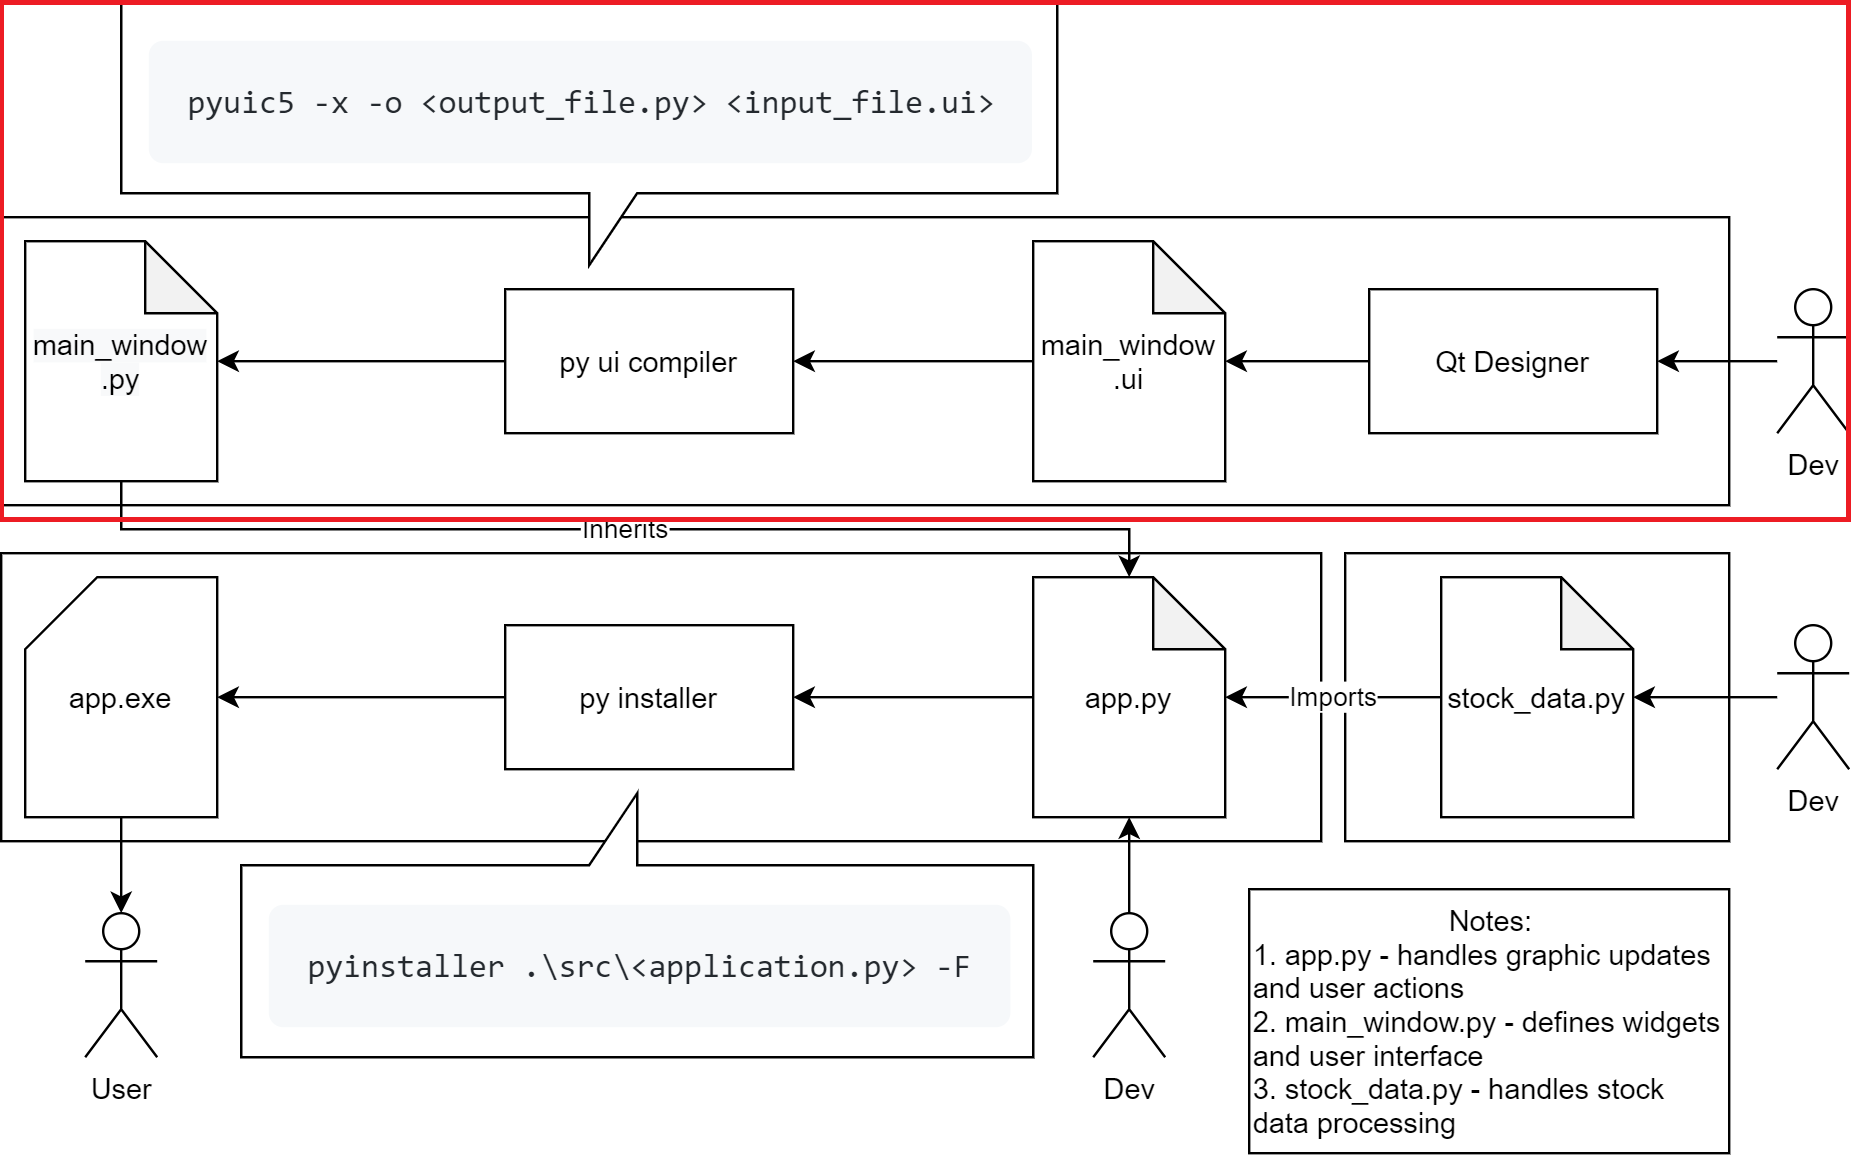
\includegraphics{../asset/img/main_window.py-process.png}

This method is \textbf{recommended} because it is user-friendly and
changes made can be seen visually on the \texttt{Qt\ Designer} itself
before it is applied. Thus, not requiring the developer to run the
python file after every changes or even knowing how do so at all.

This section of the report will now go through the 4 steps of developing
\texttt{main\_window.py} mentioned.

    \hypertarget{installing-qtdesigner}{%
\subsection{Installing QtDesigner}\label{installing-qtdesigner}}

    The installation process of QtDesigner is similar to any other
application. 1. Go to: https://build-system.fman.io/qt-designer-download
2. Click either the \texttt{Windows} or \texttt{Mac} option. Depending
on your computer's Operating System 3. Select a location for the Qt
Setup Application \texttt{.exe} to be downloaded 4. Double click on the
Qt Setup Application \texttt{.exe}and follow its installation procedure
5. Check that you have \texttt{Qt\ Designer} installed.

    \hypertarget{building-main_window.ui-using-qtdesigner}{%
\subsection{\texorpdfstring{Building \texttt{main\_window.ui} Using
QtDesigner}{Building main\_window.ui Using QtDesigner}}\label{building-main_window.ui-using-qtdesigner}}

    \hypertarget{defining-the-gui}{%
\subsubsection{Defining the GUI}\label{defining-the-gui}}

First, open \texttt{Qt\ Designer}. The following window and prompts will
appear: 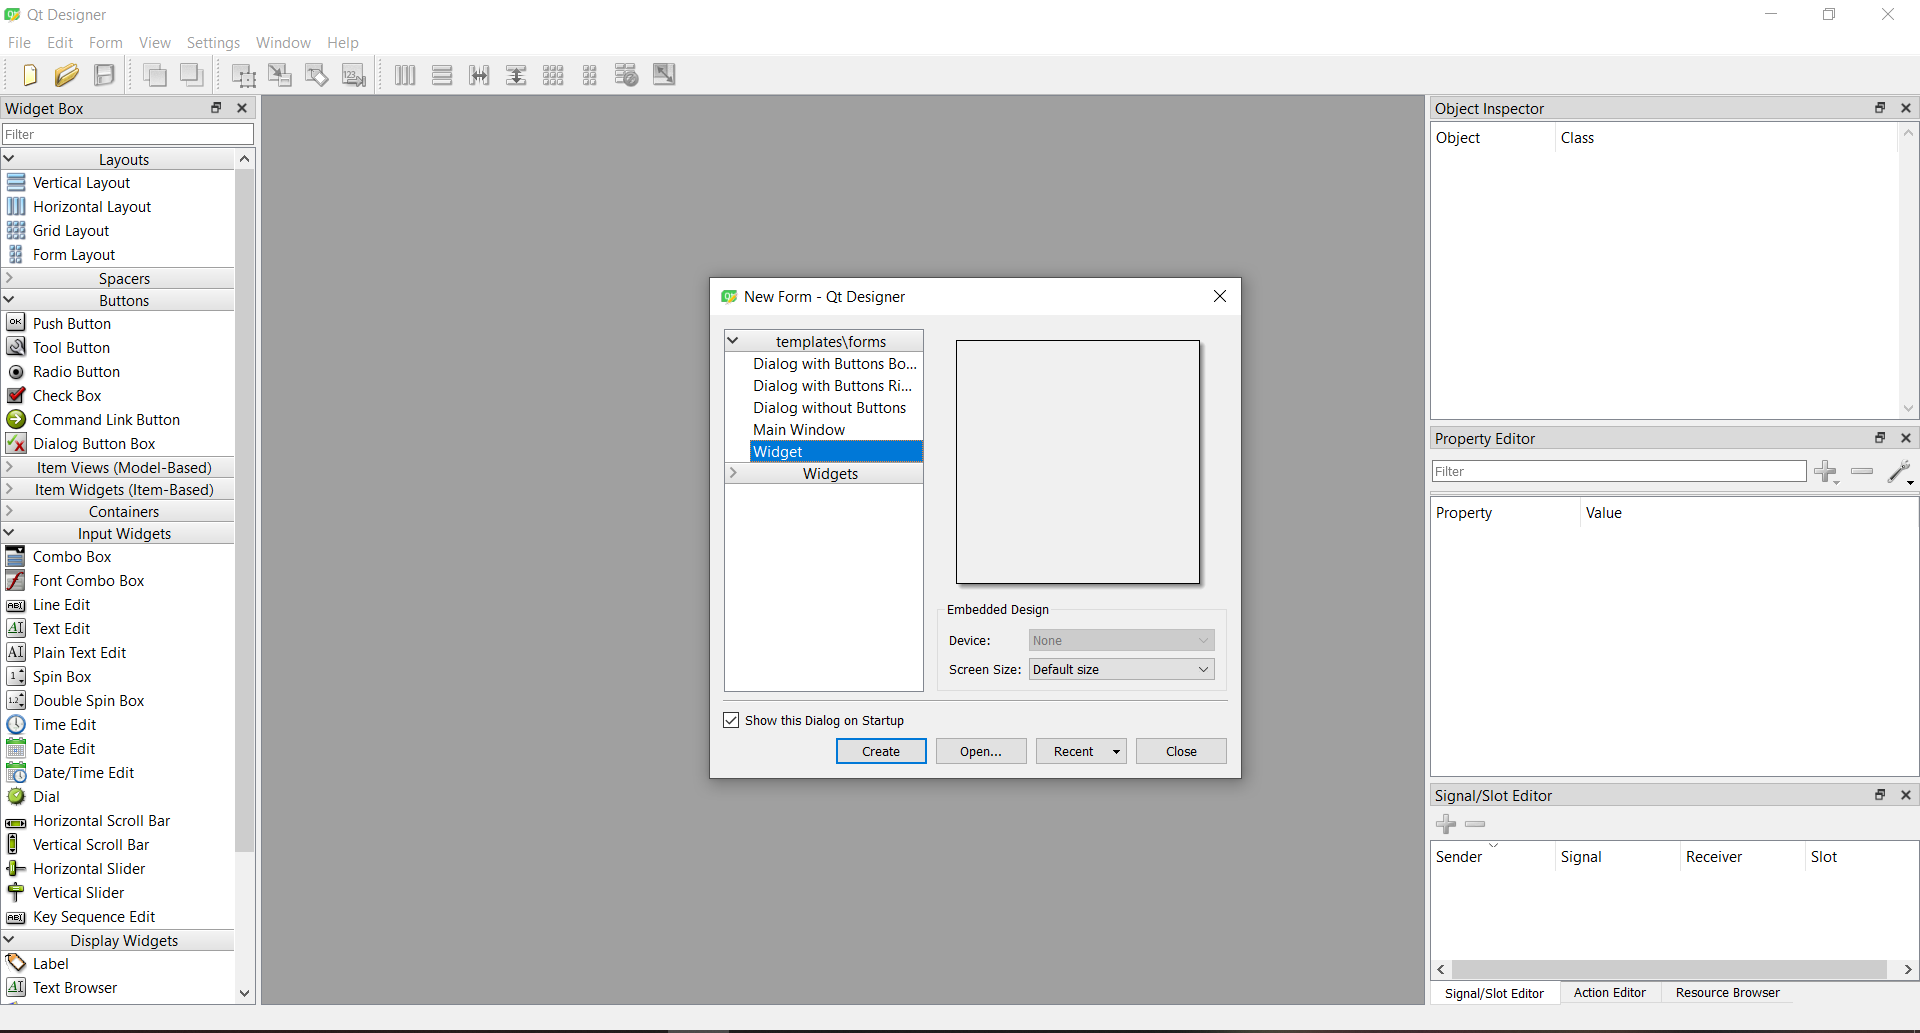
\includegraphics{../asset/img/qt-designer.png}

Choose \texttt{Widget} under the \texttt{template\textbackslash{}forms}
prompt and press the \texttt{Create} Button to begin designing
\texttt{main\_window.ui}.

This is simply a starting template of our GUI, but it is important as
the \texttt{Widget} option will later be used to inform \texttt{app.py}
of type of GUI being inherited.

    \hypertarget{defining-the-widgets-inside-the-gui}{%
\subsubsection{\texorpdfstring{Defining the \texttt{Widgets} inside the
GUI}{Defining the Widgets inside the GUI}}\label{defining-the-widgets-inside-the-gui}}

Second, start designing the \texttt{main\_window.ui} GUI as shown in the
image below: 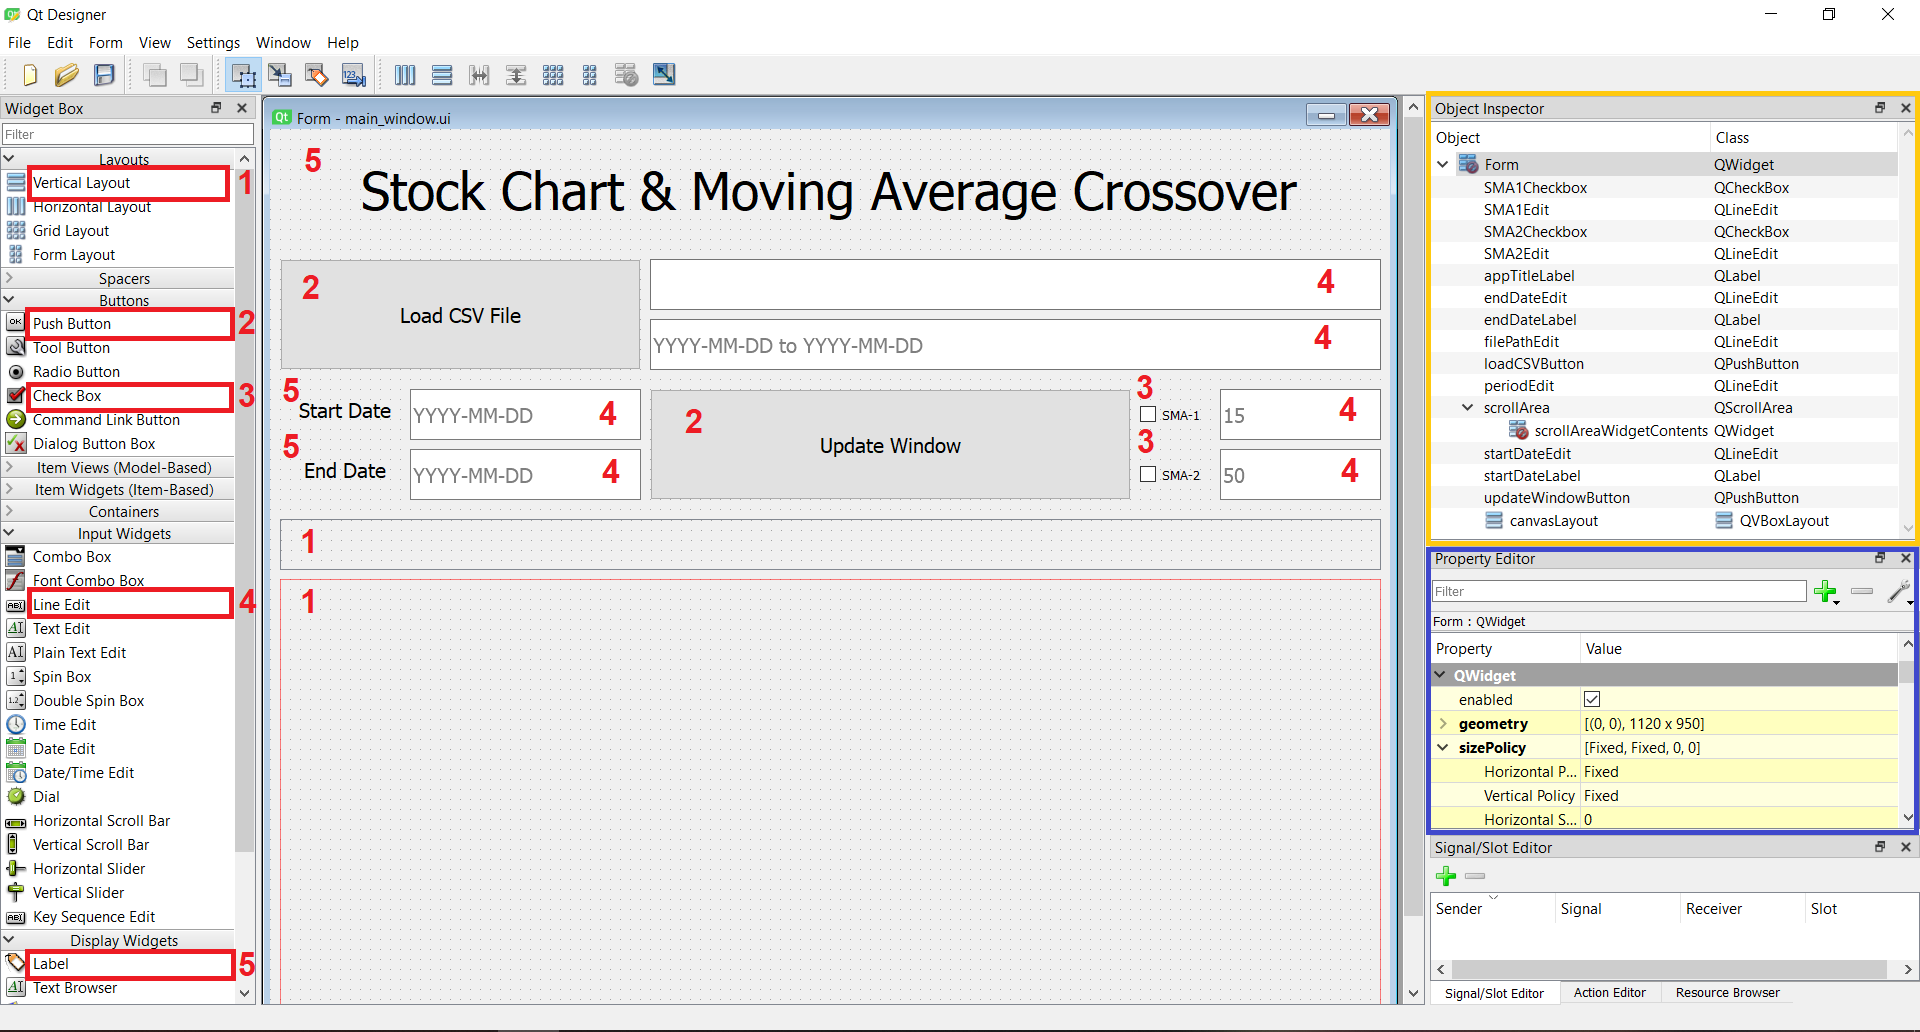
\includegraphics{../asset/img/qt-designer-gui.png}

To `design' the GUI, simply \textbf{drag and drop} the appropriate
\textbf{type} of \texttt{Widget} from the left side-bar called
\texttt{Widget\ Box} into the GUI \texttt{Widget}. This does imply that
our GUI is a \texttt{Widget} (because we specify it as such in the
\texttt{template\textbackslash{}forms} option) containing
\texttt{Widgets}.

For convenience, the \textbf{type} of the widget used to make the GUI
shown above has ben annotated with red boxes and a number to show where
to find each \textbf{type} of \texttt{Widgets} used to build the GUI.

For each \texttt{Widget} being dragged and dropped into the GUI,
remember to \textbf{name them accordingly} in the Property Box (blue
box).

These actions are what is meant by: \textgreater{} 1. Defining each
widget objects' and their names within the GUI \textgreater{} 2.
Defining the location, size and other physical attributes of each
widgets

which was mentioned at the Section \ref{main_windowpy}!

Also, do refer to the Object Inspector (yellow box) in the
\texttt{main\_window.ui} image for a list of the \textbf{names of the
widget} and their associated \texttt{Widget} \textbf{type}. For example:
name (Object): \texttt{SMA1CheckBox}, class (type): \texttt{QCheckBox}

Finally, save the \texttt{main\_window.ui} file by pressing:
\texttt{File\ \textgreater{}\ Save\ As} option on the top left hand
corner of the window.

    \hypertarget{installing-pyqt5}{%
\subsection{Installing PyQt5}\label{installing-pyqt5}}

    Installing \texttt{PyQt5} is similar to installing any other python
packages using \texttt{PIP}. Simply run the following command from the
computer's terminal:

\begin{verbatim}
pip install PyQt5
\end{verbatim}

\texttt{PyQt5} is package comprising a comprehensive set of Python
bindings for Qt v5. As part of its package, it comes with a utility
script called \texttt{pyuic5} which we can use to compile \texttt{.ui}
files created using \texttt{Qt\ Designer} into a \texttt{.py} python
module file.

    \hypertarget{compiling-main_window.ui-into-main_window.py}{%
\subsection{\texorpdfstring{Compiling \texttt{main\_window.ui} into
\texttt{main\_window.py}}{Compiling main\_window.ui into main\_window.py}}\label{compiling-main_window.ui-into-main_window.py}}

    To compile the \texttt{main\_window.ui} file into
\texttt{main\_window.py}, simply run the following command from the
computer's terminal:

\begin{verbatim}
pyuic5 -x -o .\src\main_window.py .\src\main_window.ui
\end{verbatim}

\begin{itemize}
\tightlist
\item
  The two flags \texttt{-x\ -o} are \textbf{required} for the program to
  work.
\item
  The two arguments passed are the \texttt{output} file path and the
  \texttt{input} file path.
\end{itemize}

Note: the two file paths assume that it the command is run from the
\texttt{root} directory and the \texttt{main\_window.ui} file is saved
in a directory called \texttt{src}.

    \begin{tcolorbox}[breakable, size=fbox, boxrule=1pt, pad at break*=1mm,colback=cellbackground, colframe=cellborder]
\prompt{In}{incolor}{ }{\boxspacing}
\begin{Verbatim}[commandchars=\\\{\}]

\end{Verbatim}
\end{tcolorbox}


    % Add a bibliography block to the postdoc
    
    
    
\end{document}
